% Pass options to packages before documentclass to avoid option clash
\PassOptionsToPackage{hyphens}{url}
\PassOptionsToPackage{colorlinks=true,linkcolor=blue,urlcolor=blue,citecolor=black}{hyperref}
\PassOptionsToPackage{authoryear,round}{natbib}

\documentclass[pdflatex,sn-basic]{sn-jnl}% Basic style with author-year citations

% Math packages first
\usepackage{amsmath}%
\usepackage{amssymb}%
\usepackage{amsfonts}%
\usepackage{amsthm}%
\usepackage{amsopn}%
\usepackage{amstext}%
\usepackage{mathrsfs}%
\usepackage{stmaryrd}% For llbracket, rrbracket
\usepackage{mathpartir}%

% Graphics and tables
\usepackage{graphicx}%
\DeclareGraphicsExtensions{.png,.pdf,.jpg}% PNG first, then PDF
\usepackage{subcaption}% For subfigure environment
\usepackage{caption}% For caption customization
\captionsetup{justification=raggedright, singlelinecheck=false}% Left-align all captions by default
\captionsetup[figure]{justification=centering, singlelinecheck=false}% Center-align figure captions
\usepackage{tikz}%
\usetikzlibrary{positioning,fit,backgrounds,calc,arrows.meta,decorations.pathreplacing,shapes.multipart}%
\usepackage{multirow}%
\usepackage{booktabs}%
\usepackage{pifont}% For \ding{51} (checkmark) and \ding{55} (cross)
\usepackage{tabularx}
\usepackage{array}

% Algorithm packages
\usepackage{algorithm}%
\usepackage{algorithmicx}%
\usepackage{algpseudocode}%

% Other packages
\usepackage{textcomp}% For \textregistered, \texttrademark
\usepackage{float}% For [H] option to force exact placement
\usepackage{xcolor}%
\usepackage{listings}%
\usepackage{comment}
\usepackage{placeins}% For \FloatBarrier to control figure placement
\usepackage[title]{appendix}%
\usepackage{natbib}% Options passed via \PassOptionsToPackage to avoid clash with sn-jnl
\newcolumntype{L}{>{\raggedright\arraybackslash}X}

% Define Solidity language for listings
\lstdefinelanguage{Solidity}{
  keywords={contract, function, modifier, public, private, external, internal, view, pure, payable, returns, return, if, else, for, while, require, assert, mapping, address, uint256, uint, bool, string, memory, storage, calldata, event, emit, struct, enum, constructor, msg, this, new, delete, break, continue, throw, revert},
  keywordstyle=\color{blue}\bfseries,
  ndkeywords={true, false, null, this, new},
  ndkeywordstyle=\color{darkgray}\bfseries,
  identifierstyle=\color{black},
  sensitive=true,
  comment=[l]{//},
  morecomment=[s]{/*}{*/},
  commentstyle=\color{purple}\ttfamily,
  stringstyle=\color{red}\ttfamily,
  morestring=[b]',
  morestring=[b]"
}

% Listings default settings
\lstset{
  language=Solidity,
  basicstyle=\footnotesize\ttfamily,
  backgroundcolor=\color[RGB]{248,248,248},
  numbers=left,
  numbersep=6pt
}

% Define postbreak symbol for listings
\newcommand{\lstcontinuemark}{\mbox{\textcolor{gray}{\(\hookrightarrow\)}}\space}

\theoremstyle{thmstyleone}%
\newtheorem{theorem}{Theorem}%  meant for continuous numbers
\newtheorem{proposition}[theorem]{Proposition}%
\newtheorem{lemma}[theorem]{Lemma}%
\newtheorem{corollary}[theorem]{Corollary}%
\theoremstyle{thmstyletwo}%
\newtheorem{example}{Example}%
\newtheorem{remark}{Remark}%

\theoremstyle{thmstylethree}%
\newtheorem{definition}{Definition}%

\raggedbottom

% Using author-year style to match submission guidelines
\bibpunct{(}{)}{;}{a}{,}{ } % a = author-year citations

% URL breaking settings (hyperref and url already loaded by sn-jnl.cls)
\Urlmuskip=0mu plus 1mu
\def\UrlBreaks{\do\/\do-\do\_\do\.\do\?\do\&}

\makeatletter
\renewcommand\@biblabel[1]{} % Remove numeric labels like [1]
\makeatother
\setlength{\bibsep}{0.2em}   % Space between bibliography items
\setlength{\bibhang}{2em}

% Custom math commands
\newcommand{\Abort}{\mathsf{Abort}}
\newcommand{\Norm}{\mathsf{Norm}}
\newcommand{\Ret}{\mathsf{Ret}}
\newcommand{\Env}{\mathit{Env}}


\begin{document}

\title[Solidity Intent Checker]{IntentChecker: An Intent-Model-Based Debugging Assistant for Mitigating Numeric Logic Errors in Solidity}

\author[1]{\fnm{Inseong} \sur{Jeon}}\email{iwwyou@korea.ac.kr}

\author[1]{\fnm{Sundeuk} \sur{Kim}}\email{sd\_kim@korea.ac.kr}

\author[1]{\fnm{Hyunwoo} \sur{Kim}}\email{khw0809@korea.ac.kr}

\author*[1]{\fnm{Hoh Peter} \sur{In}}\email{hoh\_in@korea.ac.kr}

\affil*[1]{\orgdiv{Department of Computer Science}, \orgname{Korea University},
\orgaddress{\street{145, Anam-ro}, \city{Seonbuk-gu}, \postcode{02841}, \state{Seoul},
\country{Republic of Korea}}}


\abstract{
Smart contract development lacks the mature debugging infrastructure available in traditional software engineering. In particular, developer intent has little direct role in the analysis available at development time.  This limitation is particularly relevant to numeric logic errors, where execution completes successfully but violates a numerical relationship intended by the developer.Existing detection tools typically evaluate source code against tool-defined vulnerability patterns, rules, or scenarios, limiting their ability to directly address numeric logic errors whose correctness depends on the intended numerical behavior of the specific code rather than on those predefined detection criteria.  This paper presents IntentChecker, a development-time value-level intent validation tool for Solidity that operates at multi-contract, single-transaction scope     and shifts the validation criterion from pre-defined vulnerability patterns to developer-defined numeric intent.  At its core is an intent model that defines the annotation syntax, formal semantics, and validation rules. Two annotation types let developers declare intent: \texttt{@During} for numerical relationships at specific program points and \texttt{@Post} for relationships at function exit. A validation engine applies the model's validation rules to the intervals computed by abstract interpretation, classifying each annotation as Satisfied, Warning, or Violated and deriving auxiliary violated-region information and a heuristic prioritization score. We evaluate IntentChecker retrospectively on real-world numeric logic errors to characterize the expressibility and validatability of reported bug-relevant intent, the associated specification and analysis costs, and its complementary role relative to existing detection tools.
}

\keywords{Solidity, Numeric Logic Error, Debugging Assistant, Value-level Intent Validation, Intent Model}

\maketitle

\section{Introduction}

The debugging toolchain available to smart contract developers remains far less mature than what traditional software engineering provides.
Our prior work, SolQDebug~\citep{solqdebug}, addressed this immaturity by performing statement-level interval-domain abstract interpretation at development time.
SolQDebug, however, goes no further than reporting raw intervals---leaving correctness judgment entirely to the developer---and its analysis remains confined to a single contract and a single transaction.
This burden is compounded by the widespread use of large language models (LLMs) such as Claude~\citep{claude}, ChatGPT~\citep{chatgpt}, and Gemini~\citep{gemini} for code generation, where the generated code is not verified against its intended behavior.

With correctness judgment left to the developer, logic errors---bugs where program behavior diverges from developer intent---are particularly hard to catch, since neither the compiler nor the runtime raises any signal.
A recent empirical study~\citep{defisecurity} confirms this difficulty: practitioners identified logic errors as the most difficult vulnerability type to detect.
In response, several tools~\citep{numscout, gptscan, sctype} explicitly target this class of bugs.
Yet they all take the source code alone as their input, operating in an auditing or testing context.
Moreover, what counts as correct in any given function is set by the developer who wrote it, so by the very definition of a logic error, detecting one requires knowing the developer's intent.
However, current tools take a different approach: they rely on a fixed set of known vulnerabilities chosen by their designers, checking code against a pre-specified set of patterns.
This mismatch is most consequential for numeric computation, which sits at the core of most smart contract code: our analysis~\citep{dappscananalysis} of 101 smart contracts from DAppSCAN-source~\citep{dappscan}, covering 1,023 non-trivial functions, finds numeric types in 82\% of them.
Logic errors are therefore most likely to arise in this space, and addressing such numeric logic errors calls for a fundamentally different kind of analysis: one that takes developer intent as direct input rather than attempting to recover it from code.

Meanwhile, developer preferences favor tools that run at development time. The same empirical study~\citep{defisecurity} reports a clear preference for IDE-integrated tools such as extensions and linters over standalone analyzers, favoring development-time tooling. It also reports a strong prioritization of low false negatives (92.3\%) over low false positives (50\%), matching the profile of sound over-approximating analyses such as abstract interpretation.
These observations together motivate a development-time tool that runs while the function is being written and lets the developer directly declare the numeric intent their contract encodes, rather than relying on pre-authored pattern catalogs to infer it.

To that end, this paper presents IntentChecker, a development-time value-level intent validation tool for Solidity built on SolQDebug and extended to a multi-contract single-transaction scope.
The intent model comprises two annotation types and a validation engine. The two annotation types cover different temporal windows of a function's execution: @During for relationships that should hold at specific program points during execution, and @Post for relationships that should hold at function exit. The validation engine, grounded in a formal denotational semantics, classifies each annotation as Satisfied, Warning, or Violated against the intervals produced by abstract interpretation, reporting the result together with a risk score on a 0--10 scale and the sub-intervals where the violation may occur.

IntentChecker is evaluated on 74 effective benchmark instances (89 collected, 15 excluded) drawn from Web3Bugs~\citep{exploitablebugs}, NumScout~\citep{numscout}, and the Greedy Contract dataset of \citet{flyinointment}.
The evaluation is organized around three research questions: whether IntentChecker can surface real-world numeric logic errors as Violated judgments at development-time latency (RQ1), what structural limitations of the analysis engine and the intent model account for the cases it cannot surface (RQ2), and how IntentChecker compares with existing detection tools along the criteria and position axes that define the design space (RQ3).
IntentChecker is positioned as a development-time complement to existing auditing-time detectors: it enables intent-driven validation during editing rather than competing with bug-pattern detectors on detection accuracy, and the RQ3 comparison is designed around this complementarity.

\smallskip
\noindent\textbf{Contributions.}
\begin{itemize}
    \item This paper defines numeric logic errors, classifies their representative patterns by abstraction level (value-level vs algorithm-level), and shows that existing detection tools share two structural constraints in addressing this class: detection criteria fixed at design time, and analysis input confined to completed source code at audit time.
    \item An intent model is presented, consisting of two annotation types and a validation engine grounded in a formal denotational semantics; the engine produces a tri-valued judgment (Satisfied / Warning / Violated) against abstract states, along with a separately computed risk score and violated region.
    \item IntentChecker is evaluated on 74 effective benchmark instances, of which 46 admit a representable numeric intent and 32 validate as Violated (median 2.11\,s per case), and is compared with ScType, GPTScan, and NumScout along the criteria and position axes to substantiate its complementary role as a development-time debugging assistant.
    \item Building on the evaluation results, this paper turns recurring patterns across the mitigated and L5 cases into three practical guidelines for authoring intent annotations: enumerating expected state effects, anchoring outputs to in-scope quantities, and expressing arithmetic intent at the mathematically ideal level.
\end{itemize}

The remainder of this paper is organized as follows.
Section~\ref{sec:background} motivates the development-time intent validation problem and surveys the structural limitations of existing detection tools.
Section~\ref{sec:design} presents the design of IntentChecker, including the deployment-unit scope, the @During/@Post intent annotations, the @IReturn debug annotation for interface return values, and the validation engine.
Section~\ref{sec:evaluation} presents evaluation results across the three research questions.
Section~\ref{sec:discussion} discusses the intent authoring effort, annotation guidelines, and remaining limitations.
Section~\ref{sec:related} reviews related work, and Section~\ref{sec:conclusion} concludes.

\section{Background}\label{sec:background}
\subsection{Numeric Logic Errors in Solidity}

Recent research has identified various numeric-related weaknesses in smart contracts~\citep{numscout,gptscan,flyinointment,exploitablebugs,defiattacks}.
Building on these findings, numeric logic errors can be defined as follows:

\begin{definition}[Numeric Logic Error]
Bugs that allow transactions to complete successfully without compile-time or runtime exceptions,
but violate the developer's intended relationships among numerical values during function execution.
\end{definition}

\begin{table}[t]
\centering
\caption{Representative single-transaction numeric logic error patterns from prior work, classified by bug abstraction level.}
\label{tab:nle-patterns}
\footnotesize
\begin{tabular}{@{}p{4.2cm}p{8.5cm}@{}}
\toprule
Pattern & Description \\
\midrule
\multicolumn{2}{@{}l}{\textit{\textbf{Value-level: the wrong number flows through a computation.}}} \\
\midrule
Div In Path~\citep{numscout}
  & Division results used in conditions can lead to unexpected control flow due to integer truncation. \\
Exchange Problem~\citep{numscout}
  & Rounding errors in exchange calculations may result in zero output despite valid input, or receiving tokens without payment. \\
Precision Loss Trend~\citep{numscout}
  & Integer division's inherent truncation tends to favor one side, potentially misaligning with protocol intent. \\
Minor Amount Retention~\citep{numscout}
  & Integer division in distributions leaves remainders unallocated to any recipient, causing permanent lock. \\
\midrule
\multicolumn{2}{@{}l}{\textit{\textbf{Algorithm-level: operations are structurally arranged in a wrong way.}}} \\
\midrule
Operator Order Issue~\citep{numscout}
  & Arithmetic order matters: $a/b*c \neq a*c/b$ due to intermediate truncation. \\
Erroneous Accounting / Wrong Interest Rate Order~\citep{gptscan, exploitablebugs}
  & Balance calculations using outdated or prematurely updated interest rates yield incorrect results. \\
Erroneous Accounting / Wrong Checkpoint Order~\citep{gptscan, exploitablebugs}
  & Incorrect ordering between state updates and checkpoints leads to reward miscalculation. \\
Inconsistent State Updates~\citep{exploitablebugs}
  & A required state variable update is omitted, causing subsequent calculations to use stale values (e.g., failing to accrue interest before a balance query). \\
Greedy Contract~\citep{flyinointment}
  & Contract can receive funds but lacks proper logic to withdraw them, causing permanent lock. \\
\bottomrule
\end{tabular}
\end{table}

These errors come in two forms.
Single-transaction errors occur within the execution of a single function call---where computation, function calls, and output generation happen in one atomic sequence.
In contrast, multiple-transaction errors only emerge through sequences of function calls, requiring analysis of inter-function dependencies and contract-level invariants.
Examples of multiple-transaction errors include Risky First Deposit and Price Oracle Manipulation~\citep{gptscan, exploitablebugs}, which manifest only through state changes accumulated across multiple function invocations.

This paper focuses on single-transaction errors---those confined to one atomic execution, though possibly spanning multiple contracts through external calls. The choice aligns with our broader goal of a development-phase debugging assistant: a single-transaction error's intended behavior is determined within the function the developer is currently writing, so the developer can declare it as input at the moment of writing. Multiple-transaction errors, whose intent spans sequences of calls authored at different times, are left to future work. Within this focus, this paper introduces a single organizing axis for the representative patterns from prior work: the bug's abstraction level (Table~\ref{tab:nle-patterns}). The axis recurs throughout the paper, later delineating IntentChecker's design target (its intent model is deliberately confined to value-level relations; \S\ref{sec:design}) and characterizing where the model reaches and where it does not (\S\ref{sec:rq1}).
\begin{itemize}
    \item \textbf{Value-level errors}---logic errors at the value level: a wrong operator, a swapped identifier, or truncation that produces a numerically incorrect result.
    \item \textbf{Algorithm-level errors}---logic errors in the structural arrangement of operations: operation ordering, an absent state update, or a missing procedure call.
\end{itemize}

The next subsection examines existing tools for numeric logic errors.

\subsection{Structural Constraints of Existing Tools}

Several tools target numeric logic errors.
NumScout~\citep{numscout} catalogs five numerical defect patterns---Div In Path,
Operator Order Issue, Exchange Problem, Precision Loss Trend, and Minor Amount
Retention---and detects them through LLM-pruned symbolic execution.
GPTScan~\citep{gptscan} targets logic vulnerabilities, including several
accounting-related patterns, by combining GPT-based scenario matching with
lightweight static analysis~\citep{slither}.
ScType~\citep{sctype} introduces a financial type system over Solidity
variables---tuples of $\langle$financial type, scaling factor, token unit,
address$\rangle$---and detects accounting errors through type checking.

These tools have meaningfully advanced automated auditing of smart-contract
logic. However, for numeric logic errors, they operate within a design space in
which the analysis criteria are primarily defined by the tool and the analyzed
program is inspected without an explicit, per-case numeric specification
provided by the developer. This gives rise to two structural constraints.

\smallskip
\noindent\textbf{(1) Detection criteria: predefined by the analysis approach.}
Each tool evaluates code against criteria established before the analyzed case:
a catalog of known defect patterns~\citep{numscout}, financial-type
constraints~\citep{sctype}, or vulnerability scenarios used to guide
LLM-assisted matching~\citep{gptscan}.
These criteria can capture recurring buggy structures effectively, but they do
not directly encode what numerical relationship the developer intended for a
particular program point or function.

For intent-dependent errors, the same surface-level computation may be correct
in one application and incorrect in another.
For example, floor division may be intentional when implementing a
rounding policy, but the same arithmetic form may constitute precision loss
when the intended relation requires rounding in the opposite direction.
Without an explicit per-case specification, the analysis must infer intended
behavior from program structure, surrounding context, or previously defined
rules and scenarios.

\smallskip
\noindent\textbf{(2) Analysis input: source-centered rather than
intent-augmented.}
Existing numeric logic error detection tools take source code as their primary
analysis input, optionally together with auxiliary information such as type
annotations or natural-language artifacts.
Their purpose is to infer whether the program matches a known defect pattern or
violates a predefined analysis rule.

This source-centered analysis model does not provide a direct channel through
which the developer can state, for the specific code under analysis, that a
particular numerical relation must hold at a particular program point.
Consequently, per-case intent is inferred rather than treated as an explicit
input to the analysis.

\smallskip
\noindent\textbf{These constraints characterize a design choice rather than a
failure of existing tools.}
The tools above are designed for their respective auditing and testing
workflows, and their effectiveness should be understood within that scope.
Our observation is instead that an analysis model based only on
tool-defined criteria cannot directly validate a developer-supplied numerical
relation unless such a relation is added to the input language.

This distinction is particularly relevant for numeric logic errors, whose
correctness often depends on application-specific numerical relationships
rather than on a universally invalid syntactic pattern.
Therefore, IntentChecker explores a complementary design point:
the developer supplies the intended numerical relation explicitly, and the
analyzer checks whether the abstract execution can establish that relation.


\subsection{Proposed Overview}\label{sec:proposed-overview}

IntentChecker extends this design space by introducing explicit numeric intent
as an analysis input and validating that intent over an interval-based abstract
execution.

\smallskip
\noindent\textbf{(1) Explicit numeric intent through developer-authored
annotations.}
IntentChecker provides two annotation forms, \texttt{@During} and
\texttt{@Post}, for expressing numerical relationships at statement-level and
function-level validation points, respectively.
These annotations define the property to be checked for the specific code
under analysis rather than relying exclusively on a tool-defined catalog of
bug patterns.

A validation engine grounded in the semantics defined in
\S\ref{sec:intent-semantics} evaluates each annotation over the intervals
computed by abstract interpretation and returns one of three judgments:
\emph{Satisfied}, \emph{Violated}, or \emph{Warning}.
Satisfied and Violated denote definite outcomes under the abstract comparison,
whereas Warning indicates that the interval abstraction is not precise enough
to establish either outcome.

In addition to this semantic judgment, the engine derives auxiliary diagnostic
information.
It reports violated sub-regions of the represented abstract value space and a
heuristic prioritization score for Warning diagnostics.
These auxiliary outputs do not affect the
Satisfied/Violated/Warning judgment; in particular, the score is not intended
as an estimate of exploit likelihood, concrete execution probability, or
application-level severity.

\smallskip
\noindent\textbf{(2) Incremental analysis during source development.}
IntentChecker is built on SolQDebug~\citep{solqdebug}, our prior
interval-based analysis framework for Solidity.
SolQDebug operates on a ``range in, range out'' principle: bounded abstract
inputs are supplied for values that cannot otherwise be determined statically,
and the analyzer propagates the resulting intervals through the program.

To support incomplete source during development, SolQDebug accepts partial
Solidity fragments through specialized grammar entry rules and incrementally
updates the control-flow graph and abstract program state.
When a source fragment is added or modified, analysis resumes from the
affected source location rather than recomputing the preceding program state.

IntentChecker reuses this infrastructure so that intent annotations can be
evaluated together with the evolving abstract state of the program.
The resulting workflow allows the declared relation to participate directly in
analysis rather than requiring the tool to reconstruct that relation solely
from the completed source code.

\smallskip
\smallskip
Together, these two components position IntentChecker as an
awareness tool rather than a detector: it does not autonomously infer
that a particular numerical computation is buggy, but instead checks
developer-supplied numeric intent and brings attention to program points where
the abstract execution violates or cannot conclusively establish the declared
relation.

Accordingly, IntentChecker assumes that the numeric relation to be checked is
provided explicitly. Discovering which relation should be specified, or
locating an unknown bug without such a specification, is outside the role
claimed for the tool. The evaluation in \S\ref{sec:evaluation} therefore
examines the expressibility and validation of bug-relevant numeric intent
rather than autonomous bug discovery.

\section{The Design of IntentChecker}\label{sec:design}

\subsection{System Architecture}

Fig.~\ref{fig:architecture} illustrates the overall architecture of IntentChecker.

\smallskip
\noindent\textbf{Input.}
IntentChecker receives three types of input:
\begin{itemize}
    \item \textbf{Source Fragment}---Solidity source fragments, such as blocks
    or statements, provided incrementally through source-code events and
    supported by SolQDebug's partial-fragment grammar
    (\S\ref{sec:proposed-overview}).

    \item \textbf{Intent Annotation}---\texttt{@During} and \texttt{@Post}
    specifications expressing intended numerical relationships at statement-
    and function-level validation points, respectively.

    \item \textbf{Debug Annotation}---analysis-input directives that supply
    bounded value ranges where the analyzer would otherwise have insufficient
    information. This category includes SolQDebug's original
    \texttt{@GlobalVar} for transaction- and block-context values,
    \texttt{@StateVar} for contract state variables, and
    \texttt{@LocalVar} for function parameters, as well as the
    \texttt{@IReturn} annotation introduced in this paper for values returned
    by interface calls.
\end{itemize}

In addition, the Analysis Module loads pre-analyzed dependency CFGs for
referenced libraries and interfaces.

\smallskip
\noindent\textbf{Output.}
For each intent annotation, IntentChecker produces:
\begin{itemize}
    \item \textbf{Result}---a semantic validation judgment of
    \emph{Satisfied}, \emph{Violated}, or \emph{Warning}.

    \item \textbf{Violated Region}---sub-intervals of the represented abstract
    value space in which the intent is definitely violated or remains
    comparison-dependent, providing developers with a localized explanation of
    a Warning result.

    \item \textbf{Risk Score}---a 0--10 heuristic prioritization score:
    $0.0$ for Satisfied, $10.0$ for Violated, and $0.1$--$9.9$ for Warning.
    For Warning results, the score is derived from the extent and shape of the
    abstract violation region and is intended only to help prioritize
    diagnostics. It does not estimate exploit likelihood, concrete execution
    probability, or application-level severity.
\end{itemize}

The Result constitutes the semantic outcome of validation, whereas the
Violated Region and Risk Score are auxiliary diagnostics derived after that
judgment has been determined. Their computation and interpretation are
described in \S\ref{sec:validation-engine}.

\begin{figure}[t]
    \centering
    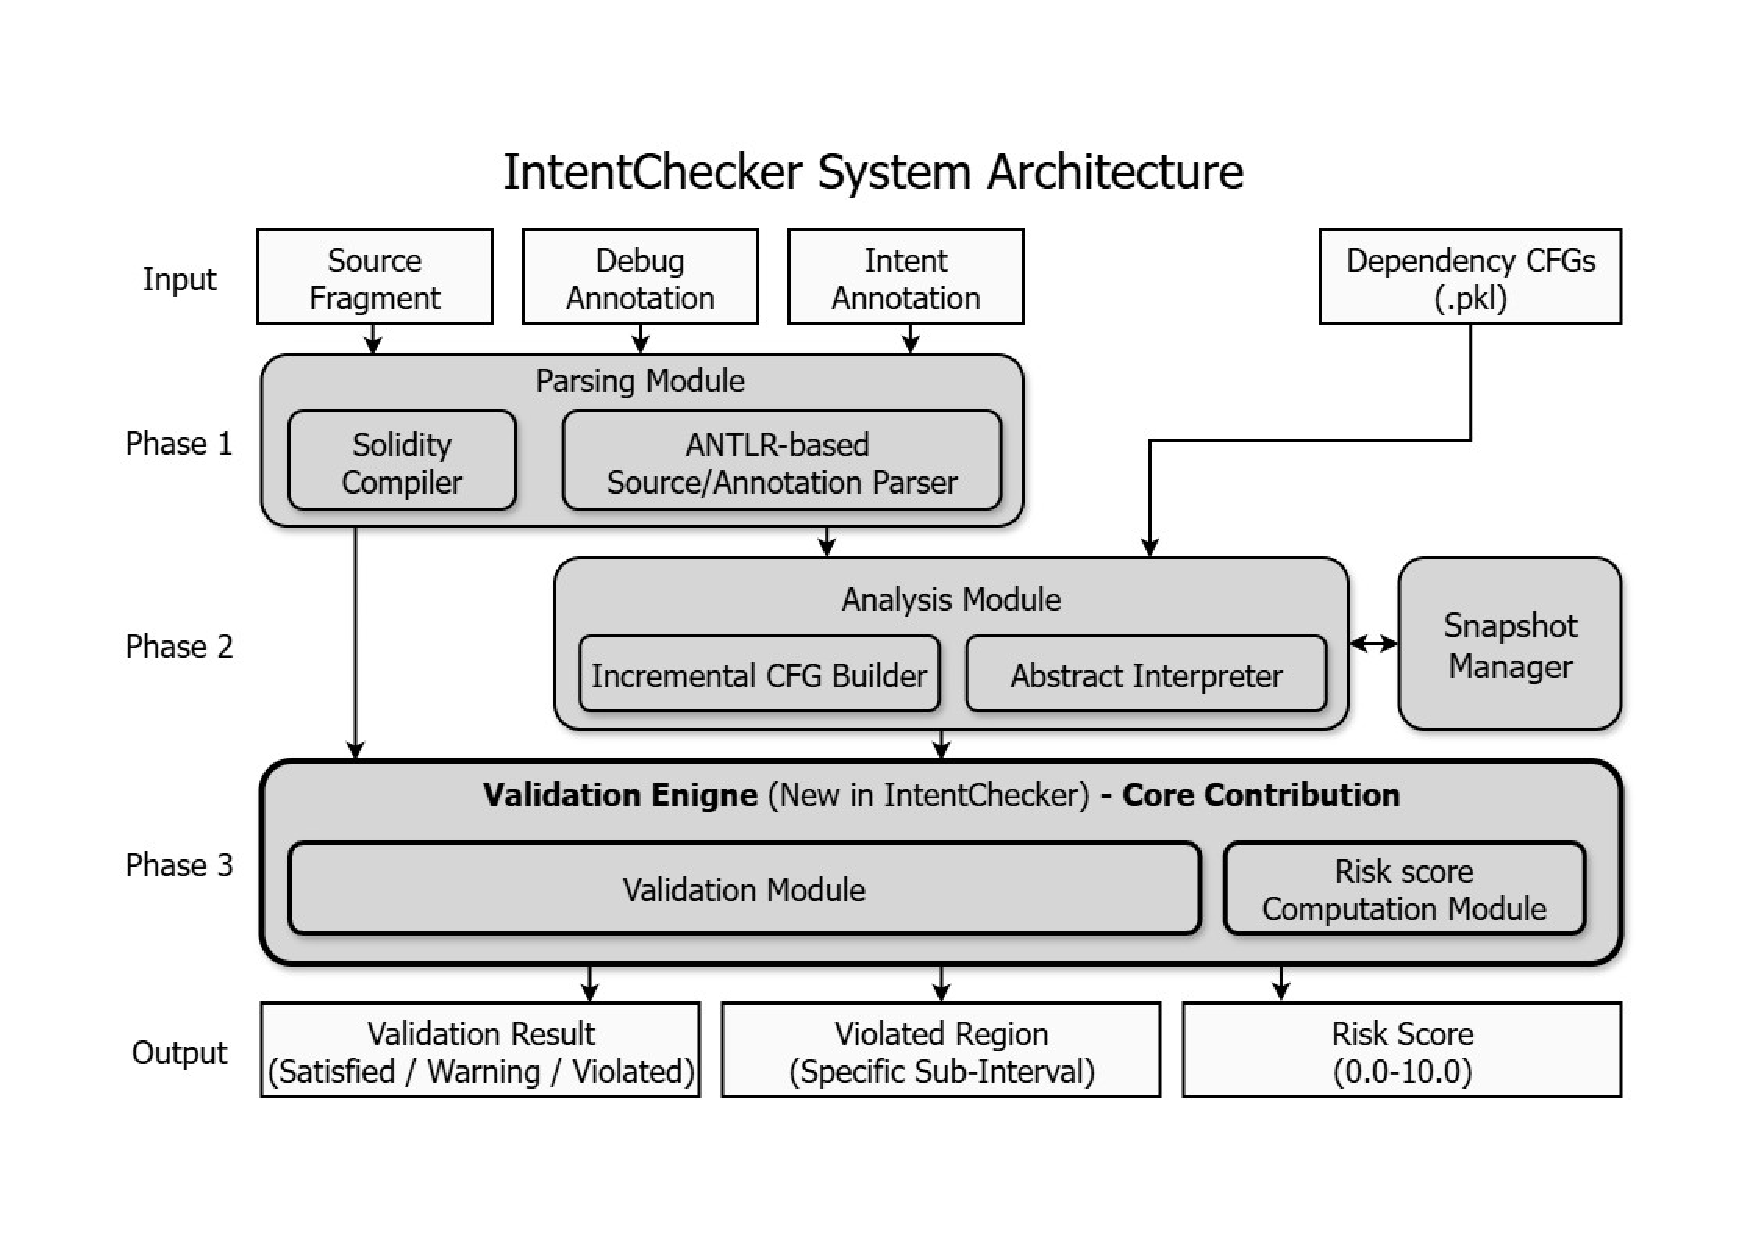
\includegraphics[width=\linewidth]{Fig1.pdf}
    \caption{System architecture of IntentChecker.}
    \label{fig:architecture}
\end{figure}

\smallskip
\noindent\textbf{Internal Modules.}
Phases~1 and~2 reuse and extend SolQDebug's analysis pipeline to accommodate
the new \texttt{@IReturn} annotation and multi-contract analysis scope, while
Phase~3 implements IntentChecker's intent-validation functionality.
\begin{itemize}
    \item \textbf{Phase~1 --- Parsing Module.}
    The Parsing Module uses ANTLR to parse Solidity source fragments together
    with intent and debug annotations. The partial-fragment grammar allows
    incomplete blocks and statements to be represented before a complete
    contract is available. Solidity units reconstructed for compiler checking
    are additionally passed to the official Solidity compiler for semantic
    validation.

    \item \textbf{Phase~2 --- Analysis Module.}
    The Analysis Module performs incremental abstract interpretation over an
    interval domain, updating the control-flow graph and abstract variable
    states as source-code events are processed. When a debug annotation is
    applied, the Snapshot Manager preserves the current analysis state,
    injects the developer-supplied interval at the target program point,
    re-analyzes the affected portion of the program, and restores the previous
    state afterward. The same mechanism is reused for \texttt{@IReturn},
    because both ordinary debug annotations and interface-return annotations
    replace an otherwise unknown abstract value with a supplied interval.

    The module also analyzes arithmetic computations in inline Yul assembly.
    Unsupported non-arithmetic assembly effects are conservatively represented
    by $\top$.

    \item \textbf{Phase~3 --- Validation Engine.}
    The Validation Engine consumes two forms of information produced by the
    preceding phases: parsed intent annotations from the Parsing Module and
    abstract variable values from the Analysis Module. For each annotation, it
    evaluates the declared numerical relationship at the corresponding
    validation context and determines a
    Satisfied/Violated/Warning judgment according to the intent semantics
    defined in \S\ref{sec:intent-semantics}. It then derives the auxiliary
    violated-region information and heuristic prioritization score without
    changing the semantic judgment.
\end{itemize}

\smallskip
\noindent\textbf{Analysis Scope.}
IntentChecker analyzes one target function at a time within a multi-contract
deployment-unit scope, extending SolQDebug's original single-contract analysis
to include inherited contract code and referenced libraries analyzed in the
target contract's execution and storage context.

Separately deployed external contracts reached through address- or
interface-typed variables remain outside this scope. Their internal storage and
callee-side state transitions are not incorporated into the target contract's
abstract state unless explicitly modeled by the analyzer. As a consequence,
values returned from external calls may evaluate to $\top$, and caller-visible
effects that are not summarized by the analysis may remain unmodeled.

The \texttt{@IReturn} annotation addresses the former problem for interface
calls whose returned values are required by downstream numerical computations.
A developer may supply a bounded interval for such a return value, allowing
analysis to continue under that abstract input instead of propagating $\top$.
This mechanism constrains the returned value only; it does not summarize
arbitrary side effects of the external call.

To limit \texttt{@IReturn} to calls for which return-value substitution does
not omit state-modifying behavior of the declared interface function, injection
is restricted to functions declared \texttt{view} or \texttt{pure}. Solidity
disallows state-modifying operations in such declared functions, whereas
non-\texttt{view}/\texttt{pure} interface calls may modify external state or
participate in re-entrant interactions and therefore require effects beyond a
return-value interval.
\subsection{Examples of Intent Annotation Usage}

This section walks through two examples to illustrate how an annotated function produces a validation judgment.
The first case demonstrates a mid-execution check via a @During annotation; the second demonstrates a post-execution check via @Post together with an @IReturn annotation for external contract state.

\smallskip
\noindent\textbf{Case 1: @During --- Operator Order Issue.}
Fig.~\ref{fig:operator-order-example} shows a token purchase function where operator precedence causes the buyer to receive fewer tokens than the exchange rate warrants.

\begin{figure}[t]
\begin{lstlisting}
// contract state: bool presell; uint256 ethRateFix;
// helper: function calculateRate() public view returns (uint256);
function buy() public payable {
    // @GlobalVar msg.value = [50000000000500000, ...]
    // @StateVar presell = true
    require(presell, "presell is closed");
    uint256 amountToBuy = msg.value / ethRateFix * calculateRate();
    // @During amountToBuy * ethRateFix >= msg.value * 250000
    balances[msg.sender] += amountToBuy;
}
\end{lstlisting}
\caption{Operator order issue in exchange rate calculation (simplified).}
\label{fig:operator-order-example}
\end{figure}

The developer's intent is that amountToBuy should satisfy the exchange-rate relation---the tokens received, times the rate denominator, should be at least the ETH paid times the rate numerator.
Because msg.value / ethRateFix truncates before multiplication, this intent is violated for non-round input amounts.
The @During annotation (line~8) captures this intent directly, and IntentChecker reports Violated.

\smallskip
\noindent\textbf{Case 2: @Post --- Erroneous Accounting.}
Fig.~\ref{fig:erroneous-accounting-example} shows a rebasing vault's mint function.
The bug is that minted proxy tokens are computed from the total vault balance (including the just-deposited amount), which inflates the shares beyond the deposited amount when the redeem rate deviates from~1.

\begin{figure}[t]
\begin{lstlisting}
// contract state: uint256 _totalSupply; mapping(address => uint256) _balances;
// address baseToken; uint256 ONE; function redeemRate() public view returns (uint256);
function mint(address to, uint256 amount)
    public override returns (uint256) {
    // @LocalVar amount = [500e18, 500e18]
    // @StateVar _totalSupply = [1000e18, 1000e18]
    // @StateVar _balances[to] = [0, 0]
    // @IReturn IERC20(baseToken).balanceOf()
    //   = [1500e18, 1500e18]
    uint256 _redeemRate = redeemRate();
    require(IERC20(baseToken).transferFrom(
        msg.sender, address(this), amount));
    uint256 baseBalance =
        IERC20(baseToken).balanceOf(address(this));
    uint256 proxy = (baseBalance * ONE) / _redeemRate;
    // @Post _balances[to] <= amount
    _mint(to, proxy);
}
\end{lstlisting}
\caption{Erroneous accounting in vault mint with inflated proxy amount (simplified).}
\label{fig:erroneous-accounting-example}
\end{figure}

The @Post \_balances[to] $\leq$ amount annotation (line~16) expresses the intent that no user should receive more shares than the tokens they deposited.
The @IReturn debug annotation (lines~8--9) injects the range $[1500\,\text{e}18, 1500\,\text{e}18]$ for the external balanceOf call (line~14), which the analyzer would otherwise evaluate as $\top$.
The transferFrom (line~11) is state-modifying and therefore cannot carry an @IReturn annotation, per the view/pure restriction described in \S\ref{sec:design}.
With these annotations, IntentChecker computes the proxy amount and finds that it exceeds amount, reporting Violated.
This example demonstrates how @IReturn enables intent validation for functions that depend on external contract state.

\smallskip
These two examples illustrate the two temporal scopes of intent validation---mid-execution checks via @During and post-execution checks via @Post.
The complete intent model supporting these annotations is defined in the following section.

\subsection{Intent Model}\label{sec:intent-model}

The denotational semantics of the intent model is built around a meaning function
\[
\mathcal{V}\llbracket \cdot \rrbracket
\;\colon\;
\mathbb{A}
\;\to\;
\bigl(\mathbb{C} \rightharpoonup \mathbb{J}\bigr),
\]
which assigns to each intent annotation $a \in \mathbb{A}$ a partial function
from validation contexts to tri-valued judgments.
The model consists of three components: the syntactic domain $\mathbb{A}$,
the semantic domain $\mathbb{C}$, and the judgment set $\mathbb{J}$.

\smallskip
\noindent\textbf{Syntactic domain.}
$\mathbb{A}$ is the set of intent annotations generated by the grammar in
\S\ref{sec:intent-semantics}, with a typical annotation denoted by $a$.
Each annotation begins with either \texttt{@During} or \texttt{@Post} and
contains one atomic intent clause.

The grammar distinguishes three classes of forms:
\begin{itemize}
    \item \textbf{@During-specific forms}, attached to an individual program
    statement and evaluated at the corresponding program point;
    \item \textbf{@Post forms}, evaluated with respect to the function-exit
    context; and
    \item \textbf{Common forms}, which may be used under either
    \texttt{@During} or \texttt{@Post}, with their reference environment
    determined by the annotation kind.
\end{itemize}

Each annotation expresses one atomic numeric obligation.
When a reported finding requires multiple independently checkable obligations,
we represent them as separate annotations rather than combining them with
annotation-level logical connectives.

\smallskip
\noindent\textbf{Semantic domain.}
We use two semantic domains:
\begin{itemize}
    \item $\Sigma$ --- the space of abstract variable environments produced by
    the interval-domain interpreter. Each $\sigma \in \Sigma$ maps program
    variables to interval-valued abstract states, including compound values
    such as arrays, mappings, and structs whose numeric leaves are represented
    by intervals.
    \item $\mathbb{C}$ --- the set of validation contexts. Each
    $\Gamma \in \mathbb{C}$ is a record containing the program-state snapshots
    and auxiliary data available when an annotation is evaluated.
\end{itemize}

\begin{table}[t]
\centering
\caption{Fields of the validation context $\Gamma \in \mathbb{C}$.
Each annotation form reads only the fields required by its semantics.}
\label{tab:validation-context}
\small
\begin{tabularx}{\linewidth}{@{} l L @{}}
\toprule
Field & Meaning \\
\midrule
$\sigma_{\text{pt}} \in \Sigma$
& abstract state at the annotated program point \\

$\sigma_{\text{before}} \in \Sigma$
& state immediately before the statement at the annotated line \\

$\sigma_{\text{assign}} \in \Sigma$
& state at the relevant variable-assignment point within the enclosing function \\

$\sigma_{\text{entry}} \in \Sigma$
& state at function entry, after parameter binding and supplied analysis inputs \\

$\sigma_{\text{exit}} \in \Sigma$
& joined state at normal function exit \\

$R : \text{Line} \rightharpoonup \text{Val}^*$
& partial map from return-statement lines to captured return values \\

$\mathcal{K}$
& statements associated with the annotated source location,
used for call-argument and \texttt{require}/\texttt{assert} lookup \\

\bottomrule
\end{tabularx}
\end{table}

\smallskip
\noindent\textbf{Field supply.}
The fields available in $\Gamma$ depend on the annotation kind:
\begin{itemize}
\item \textbf{@During}: $\sigma_{\text{pt}}$, $\sigma_{\text{before}}$,
$\sigma_{\text{assign}}$, $\sigma_{\text{entry}}$, $R$, and $\mathcal{K}$;

\item \textbf{@Post}: $\sigma_{\text{entry}}$, $\sigma_{\text{exit}}$, and $R$.
\end{itemize}

This distinction also determines the available snapshot qualifiers:
\texttt{before}, \texttt{after}, and \texttt{assign} are exposed only under
\texttt{@During}, whereas \texttt{entry} and \texttt{exit} are exposed only
under \texttt{@Post}. Unqualified references remain valid in both contexts.

\smallskip
\noindent\textbf{Judgment set.}
$\mathbb{J} = \{S,V,W\}$ is the set of tri-valued judgments:
\begin{itemize}
    \item \textbf{Satisfied} ($S$) --- every concrete state represented by the
    abstract state satisfies the annotation;
    \item \textbf{Violated} ($V$) --- every represented concrete state violates
    the annotation; and
    \item \textbf{Warning} ($W$) --- the abstract state is not precise enough to
    establish either satisfaction or violation.
\end{itemize}

For an annotation $a \in \mathbb{A}$ and validation context
$\Gamma \in \mathbb{C}$,
IntentChecker reports
$\mathcal{V}\llbracket a \rrbracket(\Gamma) \in \mathbb{J}$.
The partiality of
$\mathcal{V}\llbracket a \rrbracket$
captures that the meaning function is defined only for well-formed contexts
that provide all fields required by the selected annotation form.

The remainder of this section proceeds as follows.
Section~\ref{sec:intent-semantics} defines the syntax of $\mathbb{A}$ and the
denotational semantics of its annotation forms.
Section~\ref{sec:validation-engine} then presents the executable validation
procedures that implement these semantics.

\subsubsection{Syntax and Semantics}\label{sec:intent-semantics}

\begin{figure}[t]
\small
\begin{tabular}{@{}r@{\quad}c@{\quad}l@{\qquad}l@{}}

duringIntent
  & $\rightarrow$ & // @During duringClause & \\[2pt]

postIntent
  & $\rightarrow$ & // @Post postClause & \\[6pt]

duringClause
  & $\rightarrow$ & identifier .arg[ $n$ ] relOp intentValue$_D$
  & $(D_{\text{arg}})$ \\
  & $|$ & require feasible
  & $(D_{\text{req}})$ \\
  & $|$ & assert feasible
  & $(D_{\text{asrt}})$ \\
  & $|$ & commonClause$_D$
  & $(D_{\text{com}})$ \\[6pt]

postClause
  & $\rightarrow$ & commonClause$_P$
  & $(P_{\text{com}})$ \\[6pt]

commonClause$_k$
  & $\rightarrow$ & returnExpression relOp intentValue$_k$
  & $(C_{\text{ret}})$ \\
  & $|$ & return[$n$] relOp intentValue$_k$
  & $(C_{\text{ret}_n})$ \\
  & $|$ & intentValue$_k$ relOp PercentOf(intentValue$_k$, $p$)
  & $(C_{\text{pct}})$ \\
  & $|$ & intentValue$_k$ relOp ceil(intentValue$_k$, $d$)
  & $(C_{\text{ceil}})$ \\
  & $|$ & intentValue$_k$ relOp floor(intentValue$_k$, $d$)
  & $(C_{\text{flr}})$ \\
  & $|$ & intentValue$_k$ relOp intentValue$_k$
  & $(C_{\text{cmp}})$ \\
  & $|$ & intentValue$_k$ ${=}{>}$ intentValue$_k$
  & $(C_{\text{impl}})$ \\
  & $|$ & changed(intentValue$_k$, true $|$ false)
  & $(C_{\text{chg}})$ \\[6pt]

intentValue$_k$
  & $\rightarrow$ & arithExpr$_k$ & \\[2pt]

arithExpr$_k$
  & $\rightarrow$ &
    arithExpr$_k$ ($\ll$ $|$ $\gg$ $|$ $\ggg$) arithAdd$_k$
    $|$ arithAdd$_k$ & \\

arithAdd$_k$
  & $\rightarrow$ &
    arithAdd$_k$ (+ $|$ -) arithTerm$_k$
    $|$ arithTerm$_k$ & \\

arithTerm$_k$
  & $\rightarrow$ &
    arithTerm$_k$ (* $|$ / $|$ \%) arithExp$_k$
    $|$ arithExp$_k$ & \\

arithExp$_k$
  & $\rightarrow$ &
    arithFactor$_k$ ** arithExp$_k$
    $|$ arithFactor$_k$ & \\[2pt]

arithFactor$_D$
  & $\rightarrow$ &
    number
    $|$ [ number , number ]
    $|$ varRef
    $|$ varRef(before)
    $|$ varRef(after)
    $|$ varRef(assign)
    $|$ ( arithExpr$_D$ ) & \\

arithFactor$_P$
  & $\rightarrow$ &
    number
    $|$ [ number , number ]
    $|$ varRef
    $|$ varRef(entry)
    $|$ varRef(exit)
    $|$ ( arithExpr$_P$ ) & \\[2pt]

varRef
  & $\rightarrow$ & identifier subAccess* & \\

subAccess
  & $\rightarrow$ & . identifier $|$ [ expr ] & \\[6pt]

relOp
  & $\rightarrow$ &
    $<$ $|$ $>$ $|$ $\leq$ $|$ $\geq$ $|$ == $|$ !=
    $|$ in $|$ not in & \\

\end{tabular}

\caption{Grammar of intent annotations.
Subscripts $D$ and $P$ denote expression contexts under
\texttt{@During} and \texttt{@Post}, respectively.
Snapshot-qualified references are context-sensitive:
\texttt{before}, \texttt{after}, and \texttt{assign} are available only
under \texttt{@During}, whereas \texttt{entry} and \texttt{exit} are
available only under \texttt{@Post}.
Sub-items are tagged with rule labels
$(D_\bullet)$, $(P_\bullet)$, and $(C_\bullet)$ for reference in the text.}
\label{fig:intent-grammar}
\end{figure}

\smallskip
\noindent\textbf{Grammar overview.}
Fig.~\ref{fig:intent-grammar} gives the syntax of intent annotations,
which are embedded in single-line comments so that they coexist with Solidity
code without affecting compilation.
Intent-value expressions support arithmetic over variable references with member
and index access, numeric literals, inline intervals $[a,b]$, and the DSL helpers
\texttt{PercentOf}, \texttt{ceil}, and \texttt{floor}.

Snapshot-qualified references are context-sensitive.
Within a \texttt{@During} intent, a variable reference may be qualified with
\texttt{before}, \texttt{after}, or \texttt{assign}, referring to the
statement-level snapshots defined in Table~\ref{tab:validation-context}.
Within a \texttt{@Post} intent, a variable reference may instead be qualified
with \texttt{entry} or \texttt{exit}, referring to the function-entry and
function-exit snapshots.
An unqualified variable reference is valid in both contexts and is evaluated
against the ambient reference environment $\mathrm{ref}(\Gamma)$ defined below.
Relational operators include $<$, $>$, $\leq$, $\geq$, ==, !=,
and the membership operators \texttt{in} and \texttt{not in};
the implication operator ${=}{>}$ is a truthiness-based atomic form whose
semantics is defined below.

\smallskip
\noindent\textbf{Well-formedness.}
We write $\Gamma \vdash a : \mathbf{wf}$ to mean that annotation $a$ is
well-formed under $\Gamma$: $a$ conforms to Fig.~\ref{fig:intent-grammar},
every variable reference in $a$ resolves in the relevant field of $\Gamma$,
and all form-specific auxiliary data required by $a$ is available.
The equations below define
$\mathcal{V}\llbracket a \rrbracket(\Gamma)$
only for well-formed inputs; annotation forms whose required auxiliary data is
missing correspond to implementation error paths and lie outside the semantic
claim.

Well-formedness is orthogonal to the informativeness of the abstract inputs.
Debug annotations inherited from SolQDebug, such as \texttt{@StateVar},
\texttt{@LocalVar}, and \texttt{@IReturn}, may be used to provide bounded
intervals for otherwise-unknown values. Without such constraints, some inputs
may remain $\top$, in which case the primitives defined below may yield
$W$ even though the annotation itself is well-formed.

\smallskip
\noindent\textbf{Expression evaluation.}
Let $\mathcal{I}$ denote the set of integer intervals.
Intent-value expressions are evaluated against an abstract variable environment
$\sigma \in \Sigma$ by
\[
\text{eval} \;:\; \Sigma \times \mathit{intentValue} \;\to\; \mathcal{I}.
\]
The evaluator delegates ordinary arithmetic subexpressions to the underlying
interpreter and handles annotation-specific constructs such as
\texttt{PercentOf}, \texttt{ceil}, \texttt{floor}, and inline interval
literals $[a,b]$.
A numeric literal $n$ evaluates to the singleton interval $[n,n]$.

Rules whose left-hand sides are not themselves intent-value expressions are
handled separately.
For rule $(D_{\text{arg}})$,
$\text{arg}_n(f,\mathcal{K})$ resolves the $n$-th argument expression of the
annotated call and passes it to \text{eval}.
Rules $(C_{\text{ret}})$ and $(C_{\text{ret}_n})$ instead access the
return-summary field $R$ directly as
$R(\ell_{\text{ret}})$ and $R(\ell_{\text{ret}})[n]$.

\smallskip
\noindent\textbf{Snapshot-qualified references.}
A snapshot-qualified reference overrides the ambient environment and is evaluated
against the corresponding stored snapshot:
\[
\text{eval}(\sigma, e(\mathit{entry}))
  = \text{eval}(\sigma_{\text{entry}}, e), \qquad
\text{eval}(\sigma, e(\mathit{exit}))
  = \text{eval}(\sigma_{\text{exit}}, e),
\]
\[
\text{eval}(\sigma, e(\mathit{before}))
  = \text{eval}(\sigma_{\text{before}}, e), \qquad
\text{eval}(\sigma, e(\mathit{after}))
  = \text{eval}(\sigma_{\text{pt}}, e),
\]
\[
\text{eval}(\sigma, e(\mathit{assign}))
  = \text{eval}(\sigma_{\text{assign}}, e).
\]

Because the qualifier selects the snapshot locally for the referenced value,
snapshot-qualified references may appear anywhere inside an arithmetic expression.
For example,
\[
\mathit{debts}
  == \mathit{debts}(\mathit{entry}) + \mathit{increasingDebt}
\]
is represented as an ordinary relational comparison:
the unqualified occurrence of \textit{debts} is evaluated in
$\mathrm{ref}(\Gamma)$, while
$\mathit{debts}(\mathit{entry})$ is evaluated in
$\sigma_{\text{entry}}$.
Consequently, entry/exit and before/after comparisons do not require separate
clause-level grammar rules; they are ordinary instances of $(C_{\text{cmp}})$.

\smallskip
\noindent\textbf{Feasibility evaluator.}
To support the feasibility forms, we use the space of abstract boolean intervals
\[
\mathcal{B} = \{\{0\}, \{1\}, \{0,1\}\}
\]
and a boolean-expression evaluator
\[
\text{eval}_{\mathcal{B}}
  \;:\; \Sigma \times \text{BExpr} \;\to\; \mathcal{B},
\]
where \text{BExpr} denotes the base Solidity boolean-expression category.
The operators
$\text{cond}_{\text{req}}(\mathcal{K})$ and
$\text{cond}_{\text{asrt}}(\mathcal{K})$
extract the conditions of the annotated
\texttt{require} and \texttt{assert} statements, respectively.

\smallskip
\noindent\textbf{Comparison primitive.}
Relational annotations are grounded in
\[
\text{Cmp}^*
  \;:\; \mathcal{I} \times \text{Op} \times \mathcal{I}
  \;\to\; \mathbb{J},
\]
defined by
\[
\text{Cmp}^*(L,\mathit{op},R)
=
\begin{cases}
S & \text{if } \forall l \in L,\forall r \in R :
    l \mathrel{\mathit{op}} r, \\[2pt]
V & \text{if } \forall l \in L,\forall r \in R :
    \neg(l \mathrel{\mathit{op}} r), \\[2pt]
W & \text{otherwise.}
\end{cases}
\]
For $\mathit{op}\in\{\text{in},\text{not\,in}\}$, set membership replaces
the pointwise relation.

\smallskip
\noindent\textbf{Truthiness implication primitive.}
The implication form ${=}{>}$ is interpreted over the zero/non-zero status of
the two interval operands:
\[
\text{Impl}^*
  \;:\; \mathcal{I}\times\mathcal{I}\;\to\;\mathbb{J},
\]
with
\[
\text{Impl}^*(L,R)
=
\begin{cases}
S & \text{if } L=\{0\}, \\[2pt]
S & \text{if } 0\notin L \text{ and } 0\notin R, \\[2pt]
V & \text{if } 0\notin L \text{ and } R=\{0\}, \\[2pt]
W & \text{otherwise.}
\end{cases}
\]

\smallskip
\noindent\textbf{Feasibility primitive.}
The feasibility forms use
\[
\text{Feasible}^*
  \;:\; \mathcal{B}\;\to\;\mathbb{J},
\qquad
\text{Feasible}^*(B)
=
\begin{cases}
V & \text{if } B=\{0\}, \\
S & \text{otherwise.}
\end{cases}
\]
Thus a condition is violated only when it is provably false for every concrete
state represented by the abstract boolean interval.

\smallskip
\noindent\textbf{Meaning function.}
The meaning function
$\mathcal{V}\llbracket\cdot\rrbracket$,
introduced in \S\ref{sec:intent-model}, is defined by case analysis over the
annotation forms.
We use $e$ for an intent-value expression, $f$ for a function identifier,
and $\ell_{\text{ret}}$ for the return-statement line selected by the annotation.

\smallskip
\textbf{@During annotations.}
The forms specific to \texttt{@During} are argument comparison and feasibility.
Let $\mathcal{K}$ denote the statements at the annotated source location.
The $n$-th call argument is evaluated immediately before the call, while
feasibility is evaluated at the annotated program point:
\begin{align*}
\mathcal{V}\llbracket
f.\text{arg}[n]\ \mathit{op}\ e
\rrbracket(\Gamma)
&=
\text{Cmp}^*\bigl(
\text{eval}(\sigma_{\text{before}},\text{arg}_n(f,\mathcal{K})),
\mathit{op},
\text{eval}(\sigma_{\text{before}},e)
\bigr), \\[3pt]
%
\mathcal{V}\llbracket
\text{require feasible}
\rrbracket(\Gamma)
&=
\text{Feasible}^*\bigl(
\text{eval}_{\mathcal{B}}
(\sigma_{\text{pt}},\text{cond}_{\text{req}}(\mathcal{K}))
\bigr), \\[3pt]
%
\mathcal{V}\llbracket
\text{assert feasible}
\rrbracket(\Gamma)
&=
\text{Feasible}^*\bigl(
\text{eval}_{\mathcal{B}}
(\sigma_{\text{pt}},\text{cond}_{\text{asrt}}(\mathcal{K}))
\bigr).
\end{align*}

All \texttt{@Post} forms are common forms and therefore require no additional
annotation-specific equations.

\smallskip
\textbf{Common-form annotations.}
For forms that may appear under either annotation kind, let
\[
\mathrm{ref}(\Gamma)=
\begin{cases}
\sigma_{\text{pt}} & \text{under \texttt{@During}},\\
\sigma_{\text{exit}} & \text{under \texttt{@Post}}.
\end{cases}
\]
The common forms are then defined uniformly as
\begin{align*}
\mathcal{V}\llbracket
\text{returnExpression}\ \mathit{op}\ e
\rrbracket(\Gamma)
&=
\text{Cmp}^*\bigl(
R(\ell_{\text{ret}}),
\mathit{op},
\text{eval}(\mathrm{ref}(\Gamma),e)
\bigr), \\[3pt]
%
\mathcal{V}\llbracket
\text{return}[n]\ \mathit{op}\ e
\rrbracket(\Gamma)
&=
\text{Cmp}^*\bigl(
R(\ell_{\text{ret}})[n],
\mathit{op},
\text{eval}(\mathrm{ref}(\Gamma),e)
\bigr), \\[3pt]
%
\mathcal{V}\llbracket
e_l\ \mathit{op}\ e_r
\rrbracket(\Gamma)
&=
\text{Cmp}^*\bigl(
\text{eval}(\mathrm{ref}(\Gamma),e_l),
\mathit{op},
\text{eval}(\mathrm{ref}(\Gamma),e_r)
\bigr), \\[3pt]
%
\mathcal{V}\llbracket
e_l \Rightarrow e_r
\rrbracket(\Gamma)
&=
\text{Impl}^*\bigl(
\text{eval}(\mathrm{ref}(\Gamma),e_l),
\text{eval}(\mathrm{ref}(\Gamma),e_r)
\bigr).
\end{align*}

\smallskip
\noindent\textbf{Change detection.}
The common form $\mathrm{changed}(e,b)$ compares the value of $e$ at
function entry with its value at the evaluation boundary of the annotation.
We define the boundary environment as
\[
\mathrm{bound}(\Gamma)=
\begin{cases}
\sigma_{\mathrm{pt}} & \text{under \texttt{@During}},\\
\sigma_{\mathrm{exit}} & \text{under \texttt{@Post}}.
\end{cases}
\]

The two forms are then defined by ordinary equality and inequality comparison:
\begin{align*}
\mathcal{V}\llbracket
\mathrm{changed}(e,\mathrm{true})
\rrbracket(\Gamma)
&=
\mathrm{Cmp}^*\!\left(
    \mathrm{eval}(\sigma_{\mathrm{entry}},e),
    \neq,
    \mathrm{eval}(\mathrm{bound}(\Gamma),e)
\right), \\[3pt]
%
\mathcal{V}\llbracket
\mathrm{changed}(e,\mathrm{false})
\rrbracket(\Gamma)
&=
\mathrm{Cmp}^*\!\left(
    \mathrm{eval}(\sigma_{\mathrm{entry}},e),
    =,
    \mathrm{eval}(\mathrm{bound}(\Gamma),e)
\right).
\end{align*}

Thus, \mathrm{changed} describes a state difference between function entry
and the annotation's evaluation boundary.
It does not record whether $e$ was modified at an intermediate program point
and later restored to its entry value.
Under \texttt{@During}, the boundary is the annotated program point;
under \texttt{@Post}, it is the joined normal function-exit state.

\subsubsection{Auxiliary Diagnostics and Heuristic Prioritization}
\label{sec:validation-engine}

\begin{algorithm}[!t]
\caption{Auxiliary Diagnostics for $\mathrm{Cmp}^*$-based Annotations}
\label{alg:risk-score}
\begin{algorithmic}[1]
\State \textbf{Input:} Intervals $L$, $R$, operator $op$, judgment $j \in \mathbb{J}$
\State \textbf{Output:} $(\mathit{risk\_score},\mathit{regions})$
\State $(|T_s|,|T_v|,|T_w|) \gets \mathit{RegionSizes}(L,R,op)$
\State $\mathit{regions} \gets \mathit{ExtractViolatedRegion}(L,R,op)$
\If{$j=S$}
    \State \Return $(0.0,\mathit{regions})$
\ElsIf{$j=V$}
    \State \Return $(10.0,\mathit{regions})$
\EndIf
\State $\rho_{\mathit{sat}} \gets
       \mathit{AbstractSatisfactionRatio}(L,R,op)$
\State $\mathit{shape} \gets
       \mathit{ClassifyViolationShape}(\mathit{regions},op)$
\State $(\mathit{base},\mathit{span}) \gets
       \mathit{BandOf}(\mathit{shape})$
\State $\mathit{risk\_score}
       \gets \mathit{base}
       + (1-\rho_{\mathit{sat}})\times\mathit{span}$
\State \Return $(\mathit{risk\_score},\mathit{regions})$
\end{algorithmic}
\end{algorithm}

This subsection describes the diagnostic information produced after the
semantic judgment of \S\ref{sec:intent-semantics} has been determined.
The distinction is important: the judgment
$j\in\{S,V,W\}$ is defined by the semantics of $\mathrm{Cmp}^*$,
whereas the quantities introduced below are auxiliary outputs used to explain
and prioritize non-definite results.

For $\mathrm{Cmp}^*$-based annotations, IntentChecker derives two forms of
diagnostic information:
\begin{itemize}
    \item \textbf{violated-region information}, which identifies portions of
    the abstract operand range in which the comparison is definitely false or
    remains dependent on the other operand; and

    \item a \textbf{heuristic risk score}, which provides an ordering signal
    among Warning results using the extent and shape of the abstract
    comparison space.
\end{itemize}

Neither output changes the semantic judgment.
In particular, no cardinality-based or heuristic quantity is used to decide
whether an annotation is Satisfied, Violated, or Warning.
The score is therefore not part of the soundness claim of IntentChecker and
should not be interpreted as an estimate of exploit likelihood or
application-level severity.


\smallskip
\noindent\textbf{Step 1: Abstract-region partitioning
(Algorithm~\ref{alg:risk-score}, line 3).}
Let $L=[l_{\min},l_{\max}]$ and $R=[r_{\min},r_{\max}]$ be finite integer
intervals.
For a comparison operator $op$, the interpreter partitions the abstract values
of $L$ into three regions:
\begin{itemize}
    \item $T_s$ (\emph{definitely satisfying}):
    values $l\in L$ for which $l\mathrel{op}r$ holds for every $r\in R$;

    \item $T_v$ (\emph{definitely violating}):
    values $l\in L$ for which $l\mathrel{op}r$ fails for every $r\in R$; and

    \item $T_w$ (\emph{dependent}):
    values $l\in L$ for which the outcome depends on the particular
    value represented by $R$.
\end{itemize}

Table~\ref{tab:op-formulas} gives the corresponding conditions and
cardinalities, where
\[
n_L=l_{\max}-l_{\min}+1,
\qquad
n_R=r_{\max}-r_{\min}+1.
\]
These regions are properties of the abstract intervals.
They do not describe the frequency with which individual values occur in
concrete executions.

The definite judgment follows independently of any quantitative weighting:
$j=S$ when the comparison holds over the entire represented operand space,
$j=V$ when it fails over the entire represented operand space, and
$j=W$ otherwise.


% Keep the existing Table~\ref{tab:op-formulas} here.


\smallskip
\noindent\textbf{Step 2: Violated-region extraction
(Algorithm~\ref{alg:risk-score}, line 4).}
To provide a more concrete explanation of a Warning, the interpreter decomposes
the left-operand interval into directional components:
\begin{itemize}
    \item $L_{\mathit{lower}}$ contains values of $L$ that lie below the
    comparison boundary represented by $R$;

    \item $L_{\mathit{upper}}$ contains values of $L$ that lie above the
    comparison boundary represented by $R$; and

    \item $L_{\mathit{overlap}}$ contains values whose comparison outcome
    depends on the particular value represented by $R$.
\end{itemize}

Each component is an integer sub-interval or empty.
These regions are surfaced as diagnostic witnesses for the Warning result:
they identify where the abstract analysis finds definite or potential failure,
rather than assigning a concrete-execution probability to those failures.

% Keep the existing Table~\ref{tab:false-regions} here.


\smallskip
\noindent\textbf{Step 3: Abstract satisfaction ratio
(Algorithm~\ref{alg:risk-score}, line 10).}
For a Warning judgment, the implementation additionally computes
$\rho_{\mathit{sat}}\in[0,1]$, an \emph{abstract satisfaction ratio}.
Conceptually, for ordinary binary comparisons this quantity measures the
fraction of integer operand combinations represented by the abstract intervals
for which the comparison holds:
\[
\rho_{\mathit{sat}}(L,R,op)
=
\frac{
\left|
\{(l,r)\in L\times R \mid l\mathrel{op}r\}
\right|
}{
|L\times R|
}.
\]

The implementation evaluates this ratio in closed form rather than enumerating
all integer pairs.
For membership operators, where $R$ denotes the membership range itself,
the ratio is computed over the represented values of $L$:
\[
\rho_{\mathit{sat}}(L,R,\mathrm{in})
=
\frac{|L\cap R|}{|L|},
\qquad
\rho_{\mathit{sat}}(L,R,\mathrm{not\ in})
=
1-\frac{|L\cap R|}{|L|}.
\]

For ordering operators, the values in $T_s$ contribute fully,
the values in $T_v$ contribute nothing, and the contribution of $T_w$
is obtained by counting the satisfying integer pairs associated with each
$l\in T_w$.
Because the number of satisfying $R$-values changes arithmetically across
the contiguous warning region, this count is computed as
\[
E_w
=
\frac{(a+b)|T_w|}{2n_R},
\]
where $a$ and $b$ are the numbers of satisfying $R$-values at the two
endpoints of $T_w$.
Hence,
\[
\rho_{\mathit{sat}}
=
\frac{|T_s|+E_w}{n_L}
\]
for the corresponding ordering cases.

Importantly, $\rho_{\mathit{sat}}$ is a cardinality measure over the
\emph{abstract} operand space.
It is not a probability model for concrete executions.
The interval abstraction may contain values or operand combinations that are
not jointly reachable because correlations between program variables are not
represented.
Likewise, concrete executions need not visit the represented integer values
with equal frequency.
The ratio is therefore used only as a relative indication of how much of the
represented abstract comparison space satisfies the relation.


\smallskip
\noindent\textbf{Step 4: Violation-shape classification
(Algorithm~\ref{alg:risk-score}, line 11).}
The engine also characterizes the shape of a Warning using the directional
regions of Table~\ref{tab:false-regions}:
\begin{itemize}
    \item \textbf{Type 1} --- neither $L_{\mathit{lower}}$ nor
    $L_{\mathit{upper}}$ contains a directional violation witness;
    the uncertainty is confined to the overlap component;

    \item \textbf{Type 2} --- exactly one of
    $L_{\mathit{lower}}$ and $L_{\mathit{upper}}$ is non-empty,
    indicating a one-sided deviation; and

    \item \textbf{Type 3} --- both directional components are non-empty,
    indicating deviations on both sides.
\end{itemize}

This classification describes the \emph{shape} of the abstract violation,
not its application-level severity.
For example, a two-sided deviation is not assumed to be intrinsically more
harmful than a one-sided deviation: the consequences of under- and
over-approximation depend on the application semantics.

The implementation treats Warning results for equality and inequality
comparisons as the highest priority class by convention because non-singleton
intervals provide particularly weak information for proving equality.
This convention is a heuristic prioritization policy rather than a property of
the denotational semantics.


\smallskip
\noindent\textbf{Step 5: Heuristic warning prioritization
(Algorithm~\ref{alg:risk-score}, lines 12--13).}
Satisfied and Violated judgments are mapped to the endpoints $0.0$ and $10.0$,
respectively.
For Warning judgments, the implementation maps the violation-shape class to
one of three fixed score bands and uses
$1-\rho_{\mathit{sat}}$ to place the result within that band:
\[
\mathit{risk\_score}
=
\mathit{base}
+
(1-\rho_{\mathit{sat}})\times\mathit{span}.
\]

In the current implementation, the three bands are
$0.1$--$3.3$, $3.4$--$6.6$, and $6.7$--$9.9$.
These numerical boundaries and the ordering of the shape classes are manually
chosen heuristics.
They are not mathematically implied by the interval semantics and have not
been calibrated as probabilities or measurements of vulnerability severity.

The score is instead intended as a lightweight presentation aid for
\emph{prioritizing Warning diagnostics}.
A larger value indicates that, under this heuristic, the Warning deserves
earlier inspection because the represented abstract space contains a larger
violation component and/or a structurally broader deviation pattern.
Developers may inspect the underlying judgment and violated regions directly;
the score does not replace either diagnostic.

Accordingly, the semantic and heuristic claims of IntentChecker are separated:
the Satisfied/Violated/Warning judgment is determined solely by the abstract
comparison semantics, the violated regions and
$\rho_{\mathit{sat}}$ are deterministic properties of the represented abstract
space, and the final 0--10 score is a heuristic ranking of Warning results.
\section{Evaluation}\label{sec:evaluation}

We evaluate IntentChecker as an intent-based approach for expressing and validating numeric intent associated with numeric logic errors through three research questions examining its capabilities, associated costs, and position within the broader design space of numeric error analysis.

\begin{itemize}
    \item \textbf{RQ1 (Expressibility and Validatability)}:
    To what extent can the numeric intent associated with reported numeric logic errors be expressed and validated by IntentChecker?

    \item \textbf{RQ2 (Specification Requirements and Analysis Costs)}:
    What specification requirements and analysis costs are associated with specifying and validating numeric intent?

    \item \textbf{RQ3 (Comparison with Existing Detection Tools)}:
    How does IntentChecker compare with existing numeric logic error detection tools in terms of analysis model, coverage, and latency?
\end{itemize}

We first describe the implementation environment and benchmark dataset shared across the three research questions.

\subsection{Experimental Setup}\label{sec:setup}

\noindent\textbf{Experimental Setting.}
The evaluation environment consists of an 11th Gen Intel\textregistered{} Core\texttrademark{}
i7-11390H CPU at 3.40\,GHz with 16.0\,GB RAM, running Windows 10 (64-bit).

\noindent\textbf{Implementation and Execution.}
IntentChecker is implemented in Python~3.10 and operates directly on Solidity source code without requiring compilation or deployment.

For the evaluation, IntentChecker is executed in a controlled scripting environment that supplies source-code and annotation events to the interpreter in sequence. Source-code events incrementally update the program representation, and when a source fragment is added or modified, analysis is resumed from the affected source location rather than recomputing the preceding program state. Intent annotations register the properties to be validated at their corresponding source locations.

To provide the symbolic inputs required for analysis, IntentChecker uses the batch-annotation mechanism introduced in SolQDebug~\citep{solqdebug}. Once a complete batch annotation is provided, the analyzer evaluates the registered intents under the specified abstract state.

\smallskip
\noindent\textbf{Dataset Collection.}
We initially collect 89 real-world numeric logic error instances from three sources covering a range of numeric error patterns.
We then apply the exclusion criteria described below to obtain a final benchmark of 74 eligible instances.

\smallskip\noindent\textbf{NumScout (7 instances).}
NumScout~\citep{numscout} provides a curated collection of numeric logic errors mined from deployed BNB Smart Chain contracts.
From the 95-sample subset distributed in NumScout's official repository~\citep{numscout_dataset},
we primarily restrict the selection to contracts targeting Solidity $\geq$0.6, the version range supported by IntentChecker's front-end.
We retain one contract declaring a 0.4.x pragma because the constructs exercised by the evaluated case are nevertheless supported by the current front-end without modification.
Among the compatible cases, we select seven instances covering all five numerical defect patterns enumerated in NumScout: 
one Div In Path, two Exchange Problem, one Operator Order Issue, two Precision Loss Trend, and one Minor Amount Retention instance. 
One of the Exchange Problem instances is labeled Profit Opportunity in the repository.

\smallskip\noindent\textbf{Flyinointment (1 instance).}
From Flyinointment~\citep{flyinointment}, we include the concrete Greedy Contract example categorized as a logic weakness, as it falls within our numeric logic error scope.

\smallskip\noindent\textbf{Web3Bugs (81 instances).}
Web3Bugs~\citep{exploitablebugs} systematically collected and classified vulnerabilities reported in Code4rena audit contests.
We select cases that fall within IntentChecker's multi-contract, single-transaction analysis scope from (i) categories S6-1 through S6-4 (Erroneous Accounting) and (ii) category S3-1 (Inconsistent State Updates). 
For S3-1, we retain only cases whose root cause involves a numeric computation with a missing or stale state-variable update. 
The resulting Web3Bugs subset contains 81 instances: 72 Erroneous Accounting cases and 9 Inconsistent State Updates cases.

\begin{table}[t]
\centering
\caption{Benchmark dataset composition.}
\label{tab:dataset}
\begin{tabular*}{\linewidth}{@{\extracolsep{\fill}} l l r @{}}
\toprule
\textbf{Source} & \textbf{Error Pattern} & \textbf{Count} \\
\midrule
\multirow{5}{*}{NumScout}
  & Div In Path              & 1  \\
  & Exchange Problem         & 2  \\
  & Operator Order Issue     & 1  \\
  & Precision Loss Trend     & 2  \\
  & Minor Amount Retention   & 1  \\
\midrule
Flyinointment & Greedy Contract & 1 \\
\midrule
\multirow{2}{*}{Web3Bugs}
  & Erroneous Accounting        & 72 \\
  & Inconsistent State Updates  & 9  \\
\midrule
\textbf{Total (collected)} & & \textbf{89} \\
Excluded (see below)        & & $-15$ \\
\textbf{Effective}          & & \textbf{74} \\
\bottomrule
\end{tabular*}
\end{table}

\smallskip\noindent\textbf{Exclusions.}
Of the 89 collected instances, 15 are excluded after manual inspection because they do not satisfy our numeric-logic-error definition, fall outside the study scope, or cannot serve as distinct and reproducible benchmark instances.
The exclusion categories are:
\begin{itemize}
  \item \textbf{E1 (Source already patched, 3).} The provided source code corresponds to a post-fix version and therefore does not contain the reported bug. During provenance verification, we also inspected underlying issue-tracker records when the compiled audit report was insufficient to establish the status of the benchmark source.
  \item \textbf{E2 (Integer overflow/underflow, 2).} Under Solidity~$\geq$0.8 checked arithmetic, the reported operation causes the transaction to revert rather than producing an incorrect numeric value; we therefore exclude these cases from the numeric logic errors considered in this study.
  \item \textbf{E3 (Duplicate, 2).} Multiple audit findings refer to the same buggy code location.
  \item \textbf{E4 (Not a bug, 1).} The reported behavior was determined to be intentional rather than a valid defect based on the audit discussion and final adjudication.
  \item \textbf{E5 (Missing dependency, 2).} Required external libraries are unavailable in the audit package, preventing reconstruction of the code required for analysis.
  \item \textbf{E6 (Multi-transaction, 3).} The reported bug requires state changes across separate transactions and therefore falls outside IntentChecker's single-transaction analysis scope.
  \item \textbf{E7 (Language semantics, 1).} TThe reported behavior follows directly from Solidity's specified integer-division semantics, without an erroneous numeric implementation that violates a distinct intended relation; we therefore do not treat it as a numeric logic error under Definition 1.
  \item \textbf{E8 (Misidentified target, 1).} Provenance inspection showed that the reported defect resides in a different contract than the benchmark target, so the provided target does not contain the reported bug and cannot serve as a reproducible instance.
\end{itemize}

The remaining \textbf{74 instances} constitute the effective evaluation set.

\subsection{RQ1: Expressibility and Validatability}\label{sec:rq1}

RQ1 examines two distinct capabilities of IntentChecker. First, we ask whether the
bug-relevant numeric intent associated with a reported numeric logic error can be
represented in IntentChecker's current intent model. Second, for the cases whose
intent is expressible, we evaluate whether the analyzer can actually validate the
specified relation against the buggy implementation. Separating these two questions
is important because a relation may be representable in the annotation language even
when abstract interpretation lacks sufficient precision to establish its violation.

The evaluation is retrospective. For each benchmark instance, we reconstruct the
bug-relevant intended numeric behavior using the audit report, the buggy source code,
and, where available, the recommended or implemented fix. These sources serve only
to establish the behavior to be specified; the fix is not mechanically translated into
an annotation. Instead, we derive the least implementation-specific numeric relation
that is supported by the reported intended behavior and is sufficient to distinguish
the buggy behavior from the intended one. Accordingly, RQ1 evaluates the
representational and validation capabilities of IntentChecker given an appropriate
numeric intent specification; it does not establish that developers who are unaware
of the reported bug would independently formulate the same specification.


\subsubsection{Expressibility of Numeric Intent}\label{sec:rq1:expressibility}

We first determine whether the reconstructed numeric intent can be represented using
IntentChecker's current annotation model. A finding is considered expressible when
all independently required bug-relevant numeric obligations can be represented using
values available at supported observation points. The selected relation may take the
form of an equality, inequality or bound, an Entry/Exit or Before/After relation, a
state-change property, a return-value relation, or a relation over call arguments.
We use \texttt{@During} when the intended property concerns an intermediate program
state or statement-level effect, and \texttt{@Post} when it concerns the function's
entry/exit relationship or final state.

Expressibility is assessed independently of the subsequent abstract-interpretation
result. In particular, a relation remains expressible even if the analyzer later
returns \textit{Warning} because the abstract state is too imprecise to establish
whether the relation is satisfied or violated.

Of the 74 eligible benchmark instances, the bug-relevant numeric intent is
expressible for \textbf{46 (62.2\%)} and inexpressible for
\textbf{28 (37.8\%)}. Table~\ref{tab:rq1-expressibility} provides the
breakdown by defect type. We classify a defect as \emph{Value-level} when the
intended computation is structurally present but contains an incorrect operand,
operator, scaling term, or scalar assignment. A defect is \emph{Algorithm-level}
when the error involves a missing or additional operation, a missing state update,
or an incorrect ordering of operations.

\begin{table}[t]
\centering
\caption{Expressibility of bug-relevant numeric intent by defect type
(74 eligible instances).}
\label{tab:rq1-expressibility}
\small
\begin{tabular}{lrrr}
\toprule
\textbf{Error type} & \textbf{Expressible} & \textbf{Inexpressible} & \textbf{Total} \\
\midrule
Value     & 29 & 12 & 41 \\
Algorithm & 17 & 16 & 33 \\
\midrule
\textbf{Total} & \textbf{46} & \textbf{28} & \textbf{74} \\
\bottomrule
\end{tabular}
\end{table}


\subsubsection{Characterizing the Expressibility Boundary}\label{sec:rq1:boundary}

The results in Table~\ref{tab:rq1-expressibility} indicate that expressibility is
not limited to errors in individual arithmetic expressions. Value-level defects are
expressible in 29 of 41 cases (70.7\%), while 17 of 33 Algorithm-level defects
(51.5\%) are also expressible. Thus, missing or misordered operations can still be
captured when their intended effect can be reduced to an observable numeric relation,
such as a required state transition or an ordering-sensitive property over values
available at the relevant program point.

To identify what prevents representation in the remaining cases, we classify the
28 inexpressible findings according to four blockers. The categories describe the
specific representational obstacle rather than the developer knowledge required to
discover the bug or the precision of the subsequent analysis.

\begin{itemize}
    \item $\alpha$: a required value is obtainable only through a function call
    inside \texttt{intentValue}, and neither a known-bound substitution nor exact
    formula inlining can recover it;
    \item $\beta$: no in-scope reference to a required bug-relevant value exists;
    \item $\gamma$: the intended property is inherently structural or multi-point
    and cannot be reduced to the supported numeric relation forms; and
    \item $\delta$: the only viable observation point is architecturally unavailable
    to intent evaluation, such as a \texttt{@During} annotation whose required
    attachment point lies inside a loop body that the current engine never evaluates
    for intents.
\end{itemize}

Table~\ref{tab:rq1-blockers} summarizes the observed blockers. A finding may contain
more than one independently applicable blocker; therefore, the counts are not
mutually exclusive and sum to more than 28.

\begin{table}[t]
\centering
\caption{Reasons for inexpressibility among the 28 inexpressible findings.
Blocker counts may overlap.}
\label{tab:rq1-blockers}
\small
\begin{tabular}{c p{6.5cm} r}
\toprule
\textbf{Blocker} & \textbf{Description} & \textbf{Findings} \\
\midrule
$\alpha$ &
Required value is available only through a function call in
\texttt{intentValue}, with no applicable rescue
& 17 \\

$\beta$ &
No in-scope reference to a required value exists
& 9 \\

$\gamma$ &
Required relation is inherently structural or multi-point
& 5 \\

$\delta$ &
Required observation point is architecturally unavailable
& 2 \\
\bottomrule
\end{tabular}
\end{table}

These results suggest that the main boundary of IntentChecker's current intent model
is not simply whether the underlying defect is Value- or Algorithm-level. Rather,
expressibility depends on whether the reported intended behavior can be reduced to
numeric relations over program-observable values at supported observation points.
Algorithm-level defects remain representable when their missing or misordered behavior
has an observable numeric consequence, whereas even comparatively simple Value-level
defects may become inexpressible when a load-bearing value is unavailable to the
annotation model.

We additionally classify every eligible finding, expressible or not, as \emph{Usable}
when every value the intended relation depends on is directly referenceable at a
supported program point, and \emph{Unusable} otherwise---a purely representational
question about value availability, independent of the relation's form. Of the 74
eligible findings, \textbf{50 are Usable and 24 are Unusable}
(Table~\ref{tab:rq1-usable}).

\begin{table}[t]
\centering
\caption{Value/Algorithm defect type against Usable/Unusable, across all 74 eligible findings.}
\label{tab:rq1-usable}
\small
\begin{tabular}{lrrr}
\toprule
\textbf{Error type} & \textbf{Usable} & \textbf{Unusable} & \textbf{Total} \\
\midrule
Value     & 31 & 10 & 41 \\
Algorithm & 19 & 14 & 33 \\
\midrule
\textbf{Total} & \textbf{50} & \textbf{24} & \textbf{74} \\
\bottomrule
\end{tabular}
\end{table}

Usable and Expressible coincide almost exactly, but not quite: all 46 expressible
findings are Usable, and all 24 Unusable findings are inexpressible, yet 4 of the 28
inexpressible findings are still Usable---every required value is referenceable, but
the relation cannot be represented for another reason. These 4 findings are tagged
exclusively $\gamma$ or $\delta$, never $\alpha$ or $\beta$. This is consistent with
how the blockers are defined: $\alpha$ and $\beta$ are, by construction, failures of
value availability and therefore always coincide with Unusable, whereas $\gamma$ and
$\delta$ concern the supported relation forms and observation points rather than
which values are in scope, and so can leave a finding Usable even when it remains
inexpressible.


\subsubsection{Validation of Expressible Intent}\label{sec:rq1:validation}

We next evaluate whether the 46 expressible specifications can be validated by the
actual analyzer. For each finding, we insert the constructed target annotation into
the buggy implementation and provide batch annotations that instantiate a
bug-discriminating abstract state. We then execute IntentChecker and record the
result of the target intent check. These outcomes are obtained from actual executions
of the analyzer rather than inferred from its implementation.

We classify the validation results into three outcomes. \textit{Violated} indicates
that IntentChecker establishes that the buggy execution violates the specified
numeric intent. \textit{Warning} indicates that the intent is expressible but the
abstract state is insufficiently precise to establish either satisfaction or
violation. \textit{Unsupported} is used when the relation itself is expressible and
the observation point is valid, but the current execution model cannot represent a
state transition required to perform a discriminating validation.

As shown in Table~\ref{tab:rq1-validation}, \textbf{32 of the 46 expressible
findings (69.6\%)} produce a definite \textit{Violated} result.
A further \textbf{13 (28.3\%)} produce \textit{Warning}, while
\textbf{1 (2.2\%)} is \textit{Unsupported}.

\begin{table}[t]
\centering
\caption{Validation outcomes for the 46 expressible findings.}
\label{tab:rq1-validation}
\small
\begin{tabular}{lrr}
\toprule
\textbf{Validation outcome} & \textbf{Findings} & \textbf{\% of expressible} \\
\midrule
Violated    & 32 & 69.6\% \\
Warning     & 13 & 28.3\% \\
Unsupported &  1 &  2.2\% \\
\midrule
\textbf{Total} & \textbf{46} & \textbf{100.0\%} \\
\bottomrule
\end{tabular}
\end{table}

The single Unsupported finding depends on two independently required numeric
mechanisms. One mechanism can be validated and produces \textit{Violated}, whereas
the other depends on an implicit change to the contract's ETH balance caused by an
external call. IntentChecker's execution model does not model this external-call-
induced balance update and therefore cannot construct the state transition required
to distinguish the buggy computation from the intended relation. Under our
finding-level completeness rule, we consequently classify the finding as
\textit{Unsupported} overall rather than counting the successfully validated
mechanism alone as a finding-level \textit{Violated} result.

Table~\ref{tab:rq1-validation-by-type} further breaks down the validation outcomes by
defect type. Algorithm-level findings produce a definite violation in 14 of 17 cases
(82.4\%), whereas Value-level findings do so in 18 of 29 cases (62.1\%).
Both groups therefore contain a majority of definite violations, although the
observed difference is descriptive and should not be interpreted as evidence of a
general statistical difference between the two defect classes.

\begin{table}[t]
\centering
\caption{Validation outcomes by defect type among the 46 expressible findings.}
\label{tab:rq1-validation-by-type}
\small
\begin{tabular}{lrrrrr}
\toprule
\textbf{Error type} &
\textbf{Violated} &
\textbf{Warning} &
\textbf{Unsupported} &
\textbf{Total} &
\textbf{\% Violated} \\
\midrule
Value     & 18 & 10 & 1 & 29 & 62.1\% \\
Algorithm & 14 &  3 & 0 & 17 & 82.4\% \\
\midrule
\textbf{Total} & \textbf{32} & \textbf{13} & \textbf{1} &
\textbf{46} & \textbf{69.6\%} \\
\bottomrule
\end{tabular}
\end{table}

Overall, RQ1 shows that IntentChecker can represent the bug-relevant numeric intent
for 46 of the 74 eligible findings. Among these expressible findings, 32 yield a
definite violation when analyzed against the buggy implementation. The remaining
cases expose a separate boundary of the approach: even when an intended relation can
be stated in the intent language, abstract-interpretation precision or unmodeled
execution semantics may prevent a definite validation result. These results therefore
distinguish the representational capacity of the intent model from the validation
capability of the analyzer itself.

\subsection{RQ2: Specification Requirements and Analysis Costs}\label{sec:rq2}

RQ2 characterizes the requirements of specifying numeric intent and the computational
cost of validating it. We intentionally separate these two aspects. The first concerns
the amount and scope of program or domain information required to formulate a
bug-relevant intent specification. The second concerns the runtime cost of validating
that specification once the required analysis inputs have been supplied.

We do not interpret the structural metrics reported below as direct measurements of
developer effort. Instead, they characterize the specification profile of each finding:
how many program elements are load-bearing to the selected relation, how far the
required context extends beyond the target statement, and whether additional
protocol-specific semantics are needed. These dimensions are reported separately
rather than collapsed into a single weighted effort score.


\subsubsection{Specification Requirements}\label{sec:rq2:spec}

For each of the 46 expressible findings, we identify the program context that is
load-bearing to the derivation or justification of the selected numeric intent.
Following the dependency rules described in Section~\ref{sec:design}, we count:
(i) relevant statements,
(ii) unique relevant program values,
(iii) additional functions whose semantics must be inspected, and
(iv) additional protocol- or application-specific contracts or libraries whose
behavior is required to justify the relation.

A called function is counted once as an additional function rather than recursively
expanding its internal statements into the target function's statement count.
Likewise, generic language or library semantics are recorded as supporting context
when necessary but do not increase the protocol-specific contract/library count.
Because a small number of findings require substantially broader context than the
rest, we report medians and interquartile ranges (IQRs) rather than means.

Table~\ref{tab:rq2-profile} summarizes the resulting specification profile.
The median expressible finding depends on four relevant statements and six unique
program values. Most findings require no additional function beyond the target
function itself, and the median number of additional protocol-specific
contracts or libraries is zero.

\begin{table}[t]
\centering
\caption{Specification profile across the 46 expressible findings.}
\label{tab:rq2-profile}
\small
\begin{tabular}{lrrr}
\toprule
\textbf{Metric} & \textbf{Median} & \textbf{IQR} & \textbf{Min--Max} \\
\midrule
Relevant statements                              & 4 & 2--6 & 1--20 \\
Unique relevant values                           & 6 & 4--9 & 1--16 \\
Additional functions required                    & 0 & 0--1 & 0--3 \\
Additional protocol-specific contracts/libraries & 0 & 0--0 & 0--2 \\
\bottomrule
\end{tabular}
\end{table}

To capture not only how much context is required but also how far that context
extends from the target statement, we use the five-level context-breadth scale
defined in Section~\ref{sec:design}. Level~0 requires only the target
statement or expression; Level~1 requires additional context within the same
function; Level~2 requires another function in the same contract or library;
Level~3 requires cross-contract or cross-library context; and Level~4 requires
external protocol- or domain-specific semantics.

As shown in Table~\ref{tab:rq2-breadth}, 23 of 46 findings (50.0\%) can be
specified using only target-statement or same-function context (Levels~0--1).
A further 16 findings (34.8\%) require another function within the same
contract or library (Level~2). Only 7 findings (15.2\%) require
cross-boundary context, i.e., another contract/library or external
protocol/domain semantics (Levels~3--4).

\begin{table}[t]
\centering
\caption{Context breadth across the 46 expressible findings.}
\label{tab:rq2-breadth}
\small
\begin{tabular}{c p{5.2cm} rr}
\toprule
\textbf{Breadth} & \textbf{Meaning} & \textbf{Findings} & \textbf{\%} \\
\midrule
0 & Target statement/expression only      &  2 &  4.3\% \\
1 & Same-function context                 & 21 & 45.7\% \\
2 & Other function in same contract/library & 16 & 34.8\% \\
3 & Cross-contract/library context        &  6 & 13.0\% \\
4 & External protocol/domain specification &  1 &  2.2\% \\
\midrule
\multicolumn{2}{l}{Local (0--1)}          & 23 & 50.0\% \\
\multicolumn{2}{l}{Intra-contract (2)}    & 16 & 34.8\% \\
\multicolumn{2}{l}{Cross-boundary (3--4)} &  7 & 15.2\% \\
\bottomrule
\end{tabular}
\end{table}

The context-breadth score and the external-specification indicator capture
related but distinct properties. Context breadth records the widest category of
context required by the specification, whereas the external-specification
indicator records whether any load-bearing protocol- or domain-specific semantic
fact is required to justify the selected relation. Consequently, a finding may
depend on external protocol semantics without necessarily receiving the maximum
breadth score if its program context is otherwise narrower.

External protocol- or domain-specific semantics are required in only
\textbf{5 of 46 findings (10.9\%)}. The remaining
\textbf{41 findings (89.1\%)} can be justified from the program source together
with ordinary Solidity and generic library semantics. The audit report itself is
not counted merely because it is consulted during retrospective intent
reconstruction; however, a protocol-specific semantic fact that is load-bearing
to the selected relation and unavailable from the local source is counted as
external specification.

\begin{table}[t]
\centering
\caption{External-specification dependence across the 46 expressible findings.}
\label{tab:rq2-extspec}
\small
\begin{tabular}{lrr}
\toprule
\textbf{External specification required} & \textbf{Findings} & \textbf{\%} \\
\midrule
No  & 41 & 89.1\% \\
Yes &  5 & 10.9\% \\
\bottomrule
\end{tabular}
\end{table}

We also record how many intent clauses are required at the finding level.
A single annotation suffices for \textbf{37 of 46 findings (80.4\%)}, while
\textbf{9 findings (19.6\%)} require a multi-annotation set. Multiple annotations
are used only when the reported behavior contains independently checkable numeric
obligations that cannot be captured completely by a single relation, including
cases where the same bug-relevant mechanism applies independently to multiple
program values.

\begin{table}[t]
\centering
\caption{Annotation multiplicity across the 46 expressible findings.}
\label{tab:rq2-complexity}
\small
\begin{tabular}{lrr}
\toprule
\textbf{Annotation form} & \textbf{Findings} & \textbf{\%} \\
\midrule
Single annotation     & 37 & 80.4\% \\
Multi-annotation set  &  9 & 19.6\% \\
\bottomrule
\end{tabular}
\end{table}

Taken together, these results show that numeric-intent specification is usually
supported by relatively local program context. Half of the expressible findings
require no context beyond the target function, and fewer than one in six require
cross-contract, cross-library, or external-domain context. At the same time, the
upper ranges in Table~\ref{tab:rq2-profile} show that a smaller subset requires
substantially broader program dependencies, indicating that specification
requirements vary considerably across findings even when the final intent
annotation itself is syntactically compact.


\subsubsection{Validation Cost}\label{sec:rq2:cost}

We next measure the runtime cost of validating the 46 expressible findings after
their target intents and analysis inputs have been supplied. Each finding is
executed 10 times using a single thread. Dependency pre-analysis is excluded from
the measured interval, and both definite-\textit{Violated} and
\textit{Warning} executions are included. We use the per-case median as the
representative latency because runtime measurements may be affected by transient
system load and occasional outlier runs.

Across the 46 per-case medians, the overall median validation latency is
\textbf{2.11\,s}, with an IQR of \textbf{0.99--4.30\,s}.
The minimum per-case median is \textbf{0.39\,s}, while the maximum is
\textbf{12.99\,s}, as summarized in Table~\ref{tab:rq2-latency}.

\begin{table}[t]
\centering
\caption{IntentChecker validation latency across the 46 expressible findings
(10 runs per finding; single thread).}
\label{tab:rq2-latency}
\small
\begin{tabular}{lr}
\toprule
\textbf{Metric} & \textbf{Value} \\
\midrule
Median latency across findings & 2.11\,s \\
IQR                            & 0.99--4.30\,s \\
Min                            & 0.39\,s \\
Max                            & 12.99\,s \\
\bottomrule
\end{tabular}
\end{table}

The full per-finding distributions are provided in the supplementary material.
To assess whether 10 repetitions provide a stable representative latency, we also
compare cumulative medians obtained after 1, 3, 6, and 10 runs. This analysis is
used only as a stability check for the repetition protocol and is not treated as
an additional performance metric.

These measurements characterize the computational cost of validating an already
specified numeric intent; they do not measure the time or cognitive effort required
for a developer to formulate the specification itself. RQ2 therefore distinguishes
between structural specification requirements and analyzer runtime rather than
combining them into a single notion of ``annotation effort.'' Overall, the results
indicate that most expressible findings require relatively local specification
context, while the subsequent validation typically completes within a few seconds
under the evaluated environment.
\subsection{RQ3: Comparison with Existing Detection Tools}\label{sec:rq3}

% Title retained from the original submission -- still a comparison, but the content changes
% substantially. Old coverage scoreboard removed/heavily reconsidered: IntentChecker, ScType, GPTScan,
% and NumScout operate under different detection/validation models, so a single coverage score implies
% an unfair apples-to-apples ranking. Two-part structure below.

\subsubsection{Comparison of Analysis Models}\label{sec:rq3:models}

% Compare via design dimensions, not a coverage scoreboard:
% - specification source: developer-supplied intent / predefined rules-patterns / inferred criteria;
% - intended use phase: development-time / audit-time (post-hoc);
% - analysis objective: validating a supplied property / matching known vulnerability-error patterns;
% - property scope: general numeric relations / predefined bug classes-scenarios;
% - required prior knowledge: explicit developer-supplied specification / detector-authored criteria.
% Goal: position IntentChecker -- do not claim superior detection coverage. A compact conceptual
% comparison table is acceptable if clearly framed as a design-space table, not a detection scoreboard.

\subsubsection{Analysis Time}\label{sec:rq3:time}

% Quantitative latency comparison may remain / be strengthened -- probably the safest quantitative
% cross-tool comparison, since runtime is measurable under identical hardware/environment.
% Do NOT force all four tools over all 75 cases merely to create a coverage comparison. Define a fair
% comparison population instead, e.g. cases executable by all compared tools under their supported input
% requirements, or another clearly justified common subset.
% Report: subset-selection criterion; number of cases; repeated-run protocol; median; dispersion;
% environment; GPTScan model/API dependencies if relevant.
% Avoid selecting only the original 20 successful IntentChecker cases (obvious selection bias). If no
% clean common subset can be defined, report per-tool runtime over each tool's own valid executable cases
% and explicitly state that the distributions are not coverage-normalized.

\subsection{Threats to Validity}\label{sec:threats}

\noindent\textbf{Internal validity.}
The annotations and case classifications in RQ1 are constructed retrospectively based on reported bugs, which introduces a risk of post-hoc bias. To reduce the influence of such prior knowledge on our analysis, we separate the construction of the target specification from the assessment of its evidence provenance. We first use each audit report to identify the erroneous behavior and the bug-relevant intended numeric relation. When the report provides a recommended fix, we use it only to clarify or corroborate the reported intended behavior, rather than treating the patch itself as the target specification. Cases for which the required relation is not expressible are excluded from the subsequent provenance analysis. For each expressible case, we fix the target annotation before assessing where sufficient evidence for deriving it is available. We examine the buggy function first, including its comments, parameters, data and control flow, and sibling branches; if this local evidence is insufficient, we then examine related functions or contracts, followed by external protocol or domain knowledge when necessary. Audit reports and reported fixes are not treated as evidence in this provenance assessment. Nevertheless, because the analysis is retrospective, the procedure cannot fully eliminate post-hoc bias or establish whether independent annotators without prior knowledge of the reported bugs would derive comparable annotations. % TODO(writing-pass): tighten wording/placement below during the writing review.
Moreover, although each case's classification (Expressibility, Value/Algorithm-level, and the RQ2-A specification profile) was produced through an internal draft-and-review process, the analysis was conducted entirely by the authors without independent external verification; individual case-level judgments may therefore contain errors that a broader, independently-replicated annotation effort could surface and correct.

\smallskip
\noindent\textbf{External validity.}
The final benchmark comprises 74 numeric logic error cases collected from three complementary sources: Web3Bugs, NumScout, and the Greedy Contract example presented in Fly-in-the-Ointment. These sources cover diverse types of numeric errors that arise in real-world Solidity contracts, but they do not exhaustively cover the full space of numeric logic errors. In addition, the benchmark is constrained by IntentChecker's analysis scope: the NumScout cases are affected by the range of Solidity versions supported by IntentChecker's front-end, and the Web3Bugs cases were selected from categories relevant to the multi-contract, single-transaction analysis addressed in this study, so bugs involving state changes across multiple transactions were excluded. As a result, the distributional characteristics observed with respect to expressiveness, evidence provenance, and engine limitations may not generalize to unsupported Solidity versions, multi-transaction behavior, or numeric error types not represented in the benchmark.

\smallskip
\noindent\textbf{Construct validity.}
RQ1 evaluates two distinct properties of intent-based validation: whether a bug-relevant numeric relation can be represented by the current intent model, and whether IntentChecker can validate a supplied annotation against the buggy implementation. These properties characterize the representational and analysis capabilities of the proposed approach, but they do not directly measure its effectiveness in actual developer use. In particular, the annotations in this study are constructed retrospectively with knowledge of the reported defects. Therefore, an Expressible result shows that the bug-relevant numeric relation can be represented once that relation has been identified, and a Violated result shows that IntentChecker can expose an inconsistency once an appropriate intent specification is supplied. Neither result establishes that developers who are unaware of the reported bug would independently formulate the same or a comparable annotation, identify the relevant supporting evidence, or successfully diagnose and repair the defect. RQ2 partially addresses the specification-side dependency by characterizing the structural requirements associated with constructing and instantiating the selected intents. We report the program context required to support the specification, such as relevant statements, program values, additional functions or contracts, and context breadth, together with the analysis inputs required to instantiate the validation context, including batch annotations. These measures characterize the structural specification requirements of IntentChecker; they are not direct measurements of human annotation effort, learning curve, cognitive burden, or inter-annotator consistency. Consequently, the present evaluation cannot determine how easily developers can formulate numeric intent prospectively or how consistently independent annotators would produce comparable specifications. Evaluating these human-centered aspects would require an independent annotation or developer study.

% Internal validity / External validity / Construct validity는 위 prose로 작성 완료. 남은 항목:
%
% - Comparison validity (신규, guidance 문서 기준)
%   - cross-tool 비교는 tool마다 다른 objective/reproducibility 제약 때문에 제한적임
%   - 새 RQ3(4.4)가 direct detection-coverage scoreboard를 피하고 design dimensions(4.4.1) +
%     controlled runtime measurement(4.4.2)로 구성됨으로써 이 threat를 완화한다는 점을 명시
% - Abstract interpretation limitations (미작성)
% - 필요하면 implementation/hardware measurement validity (미작성, GPTScan 등 API 의존성 이슈 포함 가능)

\section{Discussion}\label{sec:discussion}

\subsection{Intent Annotation Guidelines}\label{sec:disc:guidelines}

Within the value-level intent model, the annotation grammar (\S\ref{sec:design}) defines what can be written. The question that remains is when a developer should write which annotation.
The 20 mitigated cases and 14 L5 expressible cases reveal a recurring pattern: the most impactful annotations express what the code does not already make explicit---an omitted state update, an unchecked relation between output and input, or the mathematical intent behind a lossy arithmetic path.
Three non-obvious guidelines are distilled from this observation.

\smallskip
\noindent\textbf{Guideline 1: Enumerate state variables a function should affect, not just those it actually affects.}
Developers naturally reason about the code they wrote---the variables they explicitly assigned, the calls they explicitly made.
Bugs of omission arise precisely from this cognitive bias: a state variable that should have been updated was simply never mentioned.
After writing a function, the developer should list the state variables whose value the function is expected to change and add at least a directional annotation (@Post var(Entry)\,$<$\,var(Exit) or @Post changed(var, true)) for each.
Crucially, this practice depends only on the developer enumerating expected effects, not on any prior knowledge of the specific bug.

\smallskip
\noindent\textbf{Guideline 2: Anchor output expectations to known quantities.}
Many functions with numeric outputs have a known relationship---a bound, an equality, or a monotonic relation---with quantities already in scope: input parameters, related state variables, or values derivable from specific input instantiations.
Encoding this relationship as a @During or @Post annotation catches wrong-implementation bugs where the code runs without error but produces a directionally wrong or out-of-bound result.
Examples include @Post \texttt{\_balances[to] <= amount} bounding the output against the transferred amount (RebaseProxy.mint), @During \texttt{\_principalWithdrawable <= \_totalLiquidityWithdrawable} comparing two related state variables (LenderPool.\_calcPrincipalWithdrawable), and @Post \texttt{returnExpression == \_balance - mapToken\_tokenAmount[\_token]} asserting the return against a state-derived formula (Pools.getAddedAmount).
Such an annotation surfaces bugs through a violated relation even when the developer cannot pre-specify the exact output value.

\smallskip
\noindent\textbf{Guideline 3: For multi-step arithmetic, annotate the result against the mathematically ideal expression, not the code as written.}
Solidity's integer division truncates at every intermediate step, and the resulting precision loss depends on the order of operations.
Code that reads amount.div(12).mul(5) may look correct, but the developer's actual intent is the mathematical value $\lfloor\text{amount} \times 5 / 12\rfloor$.
Writing the intent annotation with the multiplication-before-division ordering---@During result $\geq$ amount * 5 / 12---causes IntentChecker to compare the code's early-truncation path against a form that defers truncation to the final division, surfacing the precision gap automatically.

\subsection{Annotation Authoring Burden and Future Automation}\label{sec:disc:burden}

IntentChecker's mitigation results are conditional on the developer supplying intent and debug annotations.
This is by design: the entire approach is predicated on the developer making their intent explicit. Accordingly, IntentChecker requires direct authoring effort from the developer.

\smallskip
\noindent\textbf{Effort 1: writing intent annotations.}
The intent model requires the developer to articulate, in the grammar of @During/@Post annotations, what the function is supposed to do. This translation from a mental model of intent into grammar-expressible assertions is itself effort: the developer must decide which properties to assert at which program points and must express each assertion within the grammar's syntactic form.

\smallskip
\noindent\textbf{Effort 2: supplying debug annotations for realistic execution paths.}
Even for code whose intent is clear, IntentChecker can only analyze the path that the developer's debug annotations actually exercise.
Debug annotations require the developer to choose representative ranges for each entry-point value the function reads. Choosing ranges that miss the buggy region produces a false negative, while choosing ranges that are too wide invites widening and produces uninformative Warning judgments. Either way, Satisfied judgments hold only within the declared ranges.
This is the standard cost of any debugging paradigm---traditional debuggers also only execute the inputs the developer provides---and developers mitigate it by iteratively refining ranges when Warning results draw attention to specific sub-intervals.

\smallskip
\noindent\textbf{Future direction: LLM-assisted annotation suggestion and auto-repair.}
A natural way to lower both annotation-authoring efforts is to combine IntentChecker with a large language model that observes the same source the developer is editing.
For intent annotations, the LLM could generate candidate @During/@Post annotations from the partial code the developer is currently writing, conditioned on two paper-internal artifacts---the intent annotation guidelines (\S\ref{sec:disc:guidelines}) as structural priors and the per-case annotated benchmark as in-grammar exemplars---and present them as suggestions the developer accepts or edits.
For debug annotations, the LLM could propose representative ranges from invocation patterns visible in the project under edit and from per-pattern range exemplars in the annotated benchmark.
Such annotation suggestions can reduce the manual authoring effort for both the 20 mitigated cases and the 14 L5 cases identified in RQ2 (Fig.~\ref{fig:rq1-limitations}).
A second direction proposes in-editor code repair: when IntentChecker returns a Violated judgment, the LLM suggests edits that bring the program's actual behavior within the developer's declared intent, for them to evaluate before committing.
Both directions are left as future work, building on this paper's intent model, validation engine, guidelines (\S\ref{sec:disc:guidelines}), and per-case annotated benchmark.

\subsection{Current Limitations}\label{sec:disc:tech}

Beyond the annotation authoring burden discussed in \S\ref{sec:disc:burden}, two tool-side technical boundaries and one methodological limit of the present evaluation remain.

\smallskip
\noindent\textbf{Contract-level intent.}
IntentChecker's intent model operates on individual functions within a single transaction.
A class of numeric properties, however, constitutes contract-level intent---properties that relate quantities established by different transactions across the contract's lifetime rather than within a single function execution.
The canonical example is the ERC20 conservation property totalSupply == sum(balances): any single function execution may temporarily increment one side and not the other, but across the entire transaction history the two must agree.
Another example is the price oracle manipulation pattern, where the buggy behavior only manifests when one transaction sets up state that a later transaction reads.
Capturing contract-level intent would require tracking state across transactions and aggregating across all balance entries, both of which lie outside the current function-level, single-transaction interval-domain analysis.

\smallskip
\noindent\textbf{Unsupported Solidity constructs.}
IntentChecker's Yul support targets arithmetic computation---add, sub, mul, div/sdiv, mod/smod, exp, comparison and bitwise operators, shifts, and the modular forms mulmod/addmod---which covers the cases where inline assembly is used as a faster substitute for high-precision integer arithmetic, by far the most common use case in DeFi libraries.
However, hand-written Yul that uses memory and storage opcodes (mload/mstore, sload/sstore), control flow (if, for, switch), or function definitions falls outside the supported subset and is conservatively treated as $\top$.
The same conservative treatment applies to a small number of Solidity constructs that the abstract interpreter does not model: abi.decode from raw bytes, keccak256, and other built-ins whose results depend on opaque cryptographic operations.
Bugs whose buggy/correct distinction depends on the precise value produced by such constructs are correspondingly out of IntentChecker's reach (these account for the L3 cases in Fig.~\ref{fig:rq1-limitations}).

\smallskip
\noindent\textbf{Evaluation methodology: developer study.}
This paper evaluates IntentChecker through structural analysis---what the tool can and cannot detect (RQ1), what the intent model can and cannot express (RQ2), and how the tool compares with existing detectors (RQ3)---rather than through a developer study measuring perceived usability or annotation intuitiveness.
A controlled study with Solidity-experienced participants would answer a complementary set of questions: whether developers find the annotation syntax natural, how long annotation authoring takes in practice, and whether the tool's feedback leads to faster bug discovery than existing debugging workflows.
Meaningful results for such a study require realistic development-time conditions~\citep{defisecurity}, which in IntentChecker's current form are dominated by two confounds: the manual annotation-authoring burden described in \S\ref{sec:disc:burden}, which is specifically what the envisioned LLM-assisted suggestion layer is designed to reduce, and the analyzer coverage gaps above, which bias task selection toward cases the tool already handles.
The usability study is therefore deferred to after both the LLM-assisted annotation layer and the analyzer extensions are in place, where the study can assess the intended workflow rather than its current manual-authoring approximation.

\section{Related Works}\label{sec:related}
\subsection{Numeric Logic Error Detection in Solidity}
Logic error detection focuses on identifying discrepancies between developer intentions and actual program behavior in smart contracts.

\citep{highguard} addresses business logic violations in smart contracts by using Dynamic Condition Response (DCR) graphs
to model expected behaviors including temporal constraints, role-based access control, and inter-function dependencies.
The system monitors runtime transactions against user-provided DCR models and their function mappings,
generating violation reports when execution activities deviate from the specified business logic patterns.

\citep{smartpulse} verifies temporal properties of smart contracts by accepting user-specified Linear Temporal Logic (LTL) formulas
and attack models to check both safety and liveness properties.
The system not only detects violations but also generates concrete attack scenarios that demonstrate how the temporal properties can be violated,
providing developers with actionable insights into potential logic errors.

\citep{consolidating} enables developers to specify function and address behaviors using the ConSol syntax alongside their Solidity code,
then verifies whether the implementation adheres to these behavioral specifications and generates behavior-compliant Solidity programs without annotations.

\citep{smartinv} leverages multimodal learning to automatically infer invariants and detect machine unauditable bugs (MUBs)~\citep{exploitablebugs}
by analyzing both source code and natural language artifacts including comments, function signatures, and documented transaction scenarios.
The system employs a fine-tuned model with Tier of Thought (ToT) prompting that progressively predicts transaction contexts,
generates and ranks invariants, and ultimately identifies vulnerabilities through three-tier reasoning.

Furthermore, there are also approaches that address multiple transaction logic errors such as price manipulation~\citep{defiranger,defiguard,pomabuster,secplf,defitainter}
and flash loan attacks~\citep{defitail,midnight}.

The numeric logic error detectors above and IntentChecker differ along both axes identified in \S\ref{sec:background}.2: who authors the detection criteria and when the tool is run.
Detectors that rely on pattern catalogs, language-model inference, or type rules are all designed to run over completed code, with criteria fixed at design time and applied post-hoc.
IntentChecker is positioned earlier in time and lets the developer declare intent explicitly through annotations evaluated inside the editor, crossing both axes simultaneously.
Because the two approaches see different inputs (code only vs.\ code with declared intent) and run in different workflow stages (post-hoc audit vs.\ development-time validation), their coverage is necessarily complementary.

\subsection{Specification-based Smart Contract Verification}
Specification-based verification approaches focus on verifying general properties and correctness requirements of smart contracts rather than specific developer intentions.

\citep{scribble} provides a framework that transforms developer annotations into Solidity assertion code,
enabling testing with existing tools like MythX~\citep{mythx} and Mythril~\citep{mythril}.
The framework supports multiple annotation types including if\_succeed (conditions for successful function returns),
invariant (contract-level properties that must always hold), if\_updated (conditions checked when state variables change),
and assert (validations at specific execution points), making formal specifications accessible through familiar testing pipelines.

\citep{smartace} builds upon Scribble~\citep{scribble} to verify whether Solidity code satisfies specifications written in the Scribble language,
leveraging C-based verification tools like SeaHorn~\citep{seahorn}, libFuzzer~\citep{libfuzzer}, and KLEE~\citep{klee} by transforming smart contracts into LLVM-IR based harnesses.
The framework abstracts the $2^{160}$ possible user addresses into a small set of representative users (implicit, transient, and explicit),
enabling verification of properties that must hold for arbitrary numbers of users, such as accounting properties like
"the contract balance equals the sum of all user deposits."

\citep{idealist} verifies Solidity code using two types of annotations: specification annotations (loop invariants, call invariants, and call modifies) that developers declare as assumptions,
and verification annotations (ensures, reverts\_if, and contract invariants) that the tool checks against the implementation.
The system assumes the truth of specification annotations and uses them to verify whether the code satisfies function post-conditions,
correctly handles revert conditions, and maintains contract invariants throughout execution.

\citep{solvent} focuses on verifying liquidity properties of smart contracts through formal methods
by converting both the contract code and user-defined liquidity properties into SMT constraints.
The system then checks whether the contract satisfies these properties using SMT solvers,
generating counterexamples when violations are detected to help developers understand potential liquidity issues.

While the specification-based approaches above provide dedicated specification languages and discharge verification obligations through SMT solving, symbolic execution, or assertion injection over completed code, IntentChecker's intent model occupies a different point in the design space.
First, its annotation language targets value-level numeric intent expressed as interval-valued relationships over specific variables and program points, whereas specification-based languages above express properties as Boolean assertions over types or contract state.
Second, its tri-valued validation engine (\S\ref{sec:intent-semantics}) operates over the intervals produced by interval-domain abstract interpretation, which is light enough to run at development time as the developer writes code, whereas SMT-based and symbolic-execution-based checks are discharged as verification tasks after coding is complete.
Third, each annotation yields a graded outcome (Satisfied, Warning, or Violated) along with a risk score and the sub-intervals where the violation may occur, pointing the developer to the problematic value region rather than returning a binary verification verdict.
The two approaches are therefore complementary in specification style, verification backend, and workflow stage.

\subsection{Tools for Strengthening Security During Development Phase}
Development-phase security tools integrate vulnerability detection directly into the coding workflow, enabling developers to identify and address security issues as they write code rather than in post-development analysis.
\citep{making} presents an integrated development environment for smart contract development that combines natural language model-based code autocompletion with security validation.
The platform integrates existing static analysis tools including Oyente~\citep{oyente}, Mythril~\citep{mythril}, and Securify~\citep{securify} to provide comprehensive security reports during development workflow.

\citep{solhint} provides a Solidity linter that detects predefined vulnerability patterns including low-level calls, reentrancy, and deprecated function usage during development.
The tool enforces security best practices by checking for patterns such as proper visibility declarations, send result validation, and secure compiler version usage.

While these development-phase tools rely on design-time detection criteria for known vulnerability patterns,
IntentChecker enables developers to specify their intended numeric behaviors through annotations and validates whether the actual program execution matches the declared intent.

\section{Conclusion}\label{sec:conclusion}

This paper presents IntentChecker, a development-time value-level intent validation tool for Solidity built on SolQDebug and extended to a multi-contract single-transaction scope. The tool classifies developer-supplied @During/@Post intent annotations as Satisfied, Warning, or Violated against the abstract states produced by interval-domain analysis, grounded in a formal denotational semantics, and reports a risk score and the violated region per annotation.

On 74 effective benchmark instances drawn from Web3Bugs, NumScout, and the Greedy Contract dataset of \citet{flyinointment}, IntentChecker's intent model can represent the bug-relevant numeric relation for 46 instances (RQ1); among these, actual execution against the buggy implementation yields a Violated judgment for 32, a Warning for 13, and a single Unsupported outcome tied to an unmodeled external-call state transition. The remaining 28 instances are inexpressible, predominantly (17 of 28) because the required value is reachable only through a function call inside the annotation with no available rescue ($\alpha$), with the rest attributable to values with no in-scope reference ($\beta$, 9), inherently structural relations ($\gamma$, 5), or an architecturally unevaluated observation point ($\delta$, 2). RQ2 characterizes the specification cost of the 46 expressible instances: a median of 4 relevant statements and 6 unique program values, with half requiring no more than same-function context (breadth 0--1) and 89.1\% requiring no external protocol-specific knowledge; validation itself completes at a median of 2.11\,s per case. RQ3 then compared IntentChecker with existing detectors and empirically confirmed that their coverage and latency envelopes are bounded by both structural axes this paper identifies, namely who authors the detection criteria and when the tool is run.

These results position IntentChecker as complementary to existing detection tools: rather than competing on detection accuracy, it fills the development-time slot that auditing-time tools structurally cannot occupy. Future work targets LLM-assisted annotation suggestion and auto-repair, along with capturing contract-level intent.

\section*{Acknowledgements}
This work was supported by the Institute of Information \& communications Technology Planning \& Evaluation (IITP) grant funded by the Korean government (MSIT) (RS-2021-II210177, High Assurance of Smart Contract for Secure Software Development Life Cycle), the Technology development Program (RS-2025-25455127) funded by the Ministry of SMEs and Startups (MSS, Korea), and the ``Regional Innovation System \& Education (RISE)'' through the Seoul RISE Center, funded by the Ministry of Education (MOE) and the Seoul Metropolitan Government (2025-RISE-01-003-01).

\section*{Author Contributions}
Inseong Jeon participated in conceptualization, methodology design, system implementation, data collection, experiments, and manuscript writing. Sundeuk Kim and Hyunwoo Kim assisted in experiments, data collection and analysis, and contributed to manuscript writing. Hoh Peter In provided resources, assisted in editing the manuscript, and supervised the entire project. All authors reviewed and approved the final version of the manuscript.

\section*{Data Availability}
The benchmark of 89 real-world numeric logic error instances curated from Web3Bugs~\citep{exploitablebugs}, NumScout~\citep{numscout}, and the Greedy Contract dataset of \citet{flyinointment}, along with the IntentChecker implementation~\citep{intentchecker}, evaluation scripts, and experimental results, are available at \url{https://github.com/iwwyou/IntentChecker.git}.

\section*{Declarations}

\noindent\textbf{Competing interests} The authors declare no competing interests.

\noindent\textbf{Ethical approval} Not applicable since there are no human and/or animal studies included in this paper.


\begin{thebibliography}{99}

\bibitem[Arora et~al.(2024)]{secplf}
Arora, S., et al.: SecPLF: Secure protocols for loanable funds against oracle manipulation attacks. In: Proceedings of the 19th ACM Asia Conference on Computer and Communications Security (ASIACCS), pp. 1394--1405 (2024). https://doi.org/10.1145/3634737.3637681

\bibitem[Anthropic(2026)]{claude}
Anthropic: Claude. \url{https://www.anthropic.com/} (2026). Accessed April 2026

\bibitem[Bartoletti et~al.(2024)]{solvent}
Bartoletti, M., et al.: Solvent: liquidity verification of smart contracts. In: International Conference on Integrated Formal Methods (iFM), pp. 256--266 (2024). \url{https://doi.org/10.1007/978-3-031-76554-4_14}

\bibitem[Cadar et~al.(2008)]{klee}
Cadar, C., et al.: KLEE: unassisted and automatic generation of high-coverage tests for complex systems programs. In: OSDI, pp. 209--224 (2008). https://doi.org/10.5555/1855741.1855756

\bibitem[Chaliasos et~al.(2024)]{defisecurity}
Chaliasos, S., et al.: Smart contract and defi security tools: Do they meet the needs of practitioners?. In: Proceedings of the 46th IEEE/ACM International Conference on Software Engineering (ICSE), pp. 1--13 (2024). https://doi.org/10.1145/3597503.3623302

\bibitem[Chen et~al.(2025)]{numscout}
Chen, J., et al.: NumScout: Unveiling Numerical Defects in Smart Contracts using LLM-Pruning Symbolic Execution. IEEE Transactions on Software Engineering (2025). https://doi.org/10.1109/TSE.2025.3555622

\bibitem[NumScout(2026a)]{numscout_dataset}
NumScout: 95 Samples Experiment Dataset. \url{https://github.com/NumScout/NumScout/tree/main/Experiment/95_Samples_Run} (2026). Accessed April 2026

\bibitem[NumScout(2026b)]{numscout_semantic}
NumScout: feature detector source code (\texttt{semantic\_analysis.py}). \url{https://github.com/NumScout/NumScout/blob/main/feature_detector/semantic_analysis.py} (2026). Accessed April 2026

\bibitem[Consensys Diligence(2026a)]{mythril}
Consensys Diligence: Mythril. \url{https://github.com/ConsenSysDiligence/mythril} (2026). Accessed April 2026

\bibitem[Consensys Diligence(2026b)]{mythx}
Consensys Diligence: MythX. \url{https://mythx.io/} (2026). Accessed April 2026

\bibitem[Consensys Diligence(2026c)]{scribble}
Consensys Diligence: Scribble. \url{https://diligence.security/scribble/} (2026). Accessed April 2026

\bibitem[Eshghie et~al.(2024)]{highguard}
Eshghie, M., et al.: Highguard: Cross-chain business logic monitoring of smart contracts. In: Proceedings of the 39th IEEE/ACM International Conference on Automated Software Engineering (ASE), pp. 2378--2381 (2024). https://doi.org/10.1145/3691620.3695356

\bibitem[Feist et~al.(2019)]{slither}
Feist, J., Grieco, G., Groce, A.: Slither: A static analysis framework for smart contracts. In: 2019 IEEE/ACM 2nd International Workshop on Emerging Trends in Software Engineering for Blockchain (WETSEB), pp. 8--15 (2019). https://doi.org/10.1109/WETSEB.2019.00008

\bibitem[Gurfinkel et~al.(2015)]{seahorn}
Gurfinkel, A., et al.: The SeaHorn verification framework. In: International Conference on Computer Aided Verification, pp. 343--361 (2015). \url{https://doi.org/10.1007/978-3-319-21690-4_20}

\bibitem[Google(2026)]{gemini}
Google: Gemini. \url{https://gemini.google.com/} (2026). Accessed April 2026

\bibitem[Jeon et~al.(2026)]{solqdebug}
Jeon, I., et al.: SolQDebug: Debug solidity quickly for interactive immediacy in smart contract development. Automated Software Engineering 33(3), 86 (2026). https://doi.org/10.1007/s10515-026-00618-9

\bibitem[IntentChecker(2026a)]{intentchecker}
IntentChecker. \url{https://github.com/iwwyou/IntentChecker.git} (2026). Accessed April 2026

\bibitem[IntentChecker(2026b)]{dappscananalysis}
IntentChecker: DAppSCAN contract analysis dataset. \url{https://github.com/iwwyou/IntentChecker/blob/main/evaluation/DappSCAN_contract_analysis/contract_analysis_table.xlsx} (2026). Accessed April 2026

\bibitem[IntentChecker(2026c)]{rq2supp}
IntentChecker: RQ2 supplementary material---L4/L5 case classifications and annotations. \url{https://github.com/iwwyou/IntentChecker/tree/main/evaluation/RQ2} (2026). Accessed April 2026

\bibitem[IntentChecker(2026d)]{rq1supp}
IntentChecker: RQ1 supplementary material---per-case annotation plans and rationale. \url{https://github.com/iwwyou/IntentChecker/tree/main/evaluation/RQ1/annotation_plans.md} (2026). Accessed April 2026

\bibitem[Kong et~al.(2023)]{defitainter}
Kong, Q., et al.: Defitainter: Detecting price manipulation vulnerabilities in defi protocols. In: Proceedings of the 32nd ACM SIGSOFT International Symposium on Software Testing and Analysis (ISSTA), pp. 1144--1156 (2023). https://doi.org/10.1145/3597926.3598124

\bibitem[Li et~al.(2025)]{defitail}
Li, X., et al.: Penetrating the hostile: Detecting defi protocol exploits through cross-contract analysis. IEEE Transactions on Information Forensics and Security 20, 11759--11774 (2025). https://doi.org/10.1109/TIFS.2025.3626979

\bibitem[LLVM(2026)]{libfuzzer}
LLVM: libFuzzer. \url{https://llvm.org/docs/LibFuzzer.html} (2026). Accessed April 2026

\bibitem[Luu et~al.(2016)]{oyente}
Luu, L., et al.: Making smart contracts smarter. In: Proceedings of the 2016 ACM SIGSAC Conference on Computer and Communications Security (CCS), pp. 254--269 (2016). https://doi.org/10.1145/2976749.2978309

\bibitem[Nguyen et~al.(2023)]{idealist}
Nguyen, T.D., et al.: An idealist's approach for smart contract correctness. In: International Conference on Formal Engineering Methods, pp. 11--28 (2023). \url{https://doi.org/10.1007/978-981-99-7584-6_2}

\bibitem[OpenAI(2026)]{chatgpt}
OpenAI: ChatGPT. \url{https://chatgpt.com/} (2026). Accessed April 2026

\bibitem[Pearson(2026)]{pearson_r}
Pearson correlation coefficient. \url{https://en.wikipedia.org/wiki/Pearson_correlation_coefficient} (2026). Accessed April 2026

\bibitem[Protofire(2026)]{solhint}
Protofire: Solhint. \url{https://github.com/protofire/solhint} (2026). Accessed April 2026

\bibitem[Ramezany et~al.(2023)]{midnight}
Ramezany, S., Setthawong, R., Setthawong, P.: Midnight: An Efficient Event-driven EVM Transaction Security Monitoring Approach For Flash Loan Detection. In: Proceedings of the 2023 20th International Joint Conference on Computer Science and Software Engineering (JCSSE), pp. 237--241 (2023). https://doi.org/10.1109/JCSSE58229.2023.10201970

\bibitem[Ren et~al.(2021)]{making}
Ren, M., et al.: Making smart contract development more secure and easier. In: Proceedings of the 29th ACM Joint Meeting on European Software Engineering Conference and Symposium on the Foundations of Software Engineering (ESEC/FSE), pp. 1360--1370 (2021). https://doi.org/10.1145/3468264.3473929

\bibitem[Soud et~al.(2024)]{flyinointment}
Soud, M., Liebel, G., Hamdaqa, M.: A fly in the ointment: an empirical study on the characteristics of Ethereum smart contract code weaknesses. Empirical Software Engineering 29(1), 13 (2024). https://doi.org/10.1007/s10664-023-10398-5

\bibitem[Stephens et~al.(2021)]{smartpulse}
Stephens, J., et al.: SmartPulse: automated checking of temporal properties in smart contracts. In: Proceedings of the 2021 IEEE Symposium on Security and Privacy (SP), pp. 555--571 (2021). https://doi.org/10.1109/SP40001.2021.00085

\bibitem[Sun et~al.(2024)]{gptscan}
Sun, Y., et al.: Gptscan: Detecting logic vulnerabilities in smart contracts by combining gpt with program analysis. In: Proceedings of the IEEE/ACM 46th International Conference on Software Engineering (ICSE), pp. 1--13 (2024). https://doi.org/10.1145/3597503.3639117

\bibitem[GPTScan(2023)]{gptscan_web3bugs}
GPTScan: Web3Bugs per-contest evaluation results. \url{https://github.com/MetaTrustLabs/GPTScan-Web3Bugs} (2023). Accessed April 2026

\bibitem[Tsankov et~al.(2018)]{securify}
Tsankov, P., et al.: Securify: Practical security analysis of smart contracts. In: Proceedings of the 2018 ACM SIGSAC Conference on Computer and Communications Security (CCS), pp. 67--82 (2018). https://doi.org/10.1145/3243734.3243780

\bibitem[Wang et~al.(2024a)]{defiguard}
Wang, D., et al.: Defiguard: A price manipulation detection service in defi using graph neural networks. IEEE Transactions on Services Computing (2024). https://doi.org/10.1109/TSC.2024.3489439

\bibitem[Wang et~al.(2024b)]{smartinv}
Wang, S.J., Pei, K., Yang, J.: Smartinv: Multimodal learning for smart contract invariant inference. In: Proceedings of the 2024 IEEE Symposium on Security and Privacy (SP), pp. 2217--2235 (2024). https://doi.org/10.1109/SP54263.2024.00126

\bibitem[Wei et~al.(2024)]{consolidating}
Wei, G., et al.: Consolidating Smart Contracts with Behavioral Contracts. Proceedings of the ACM on Programming Languages 8(PLDI), 965--989 (2024). https://doi.org/10.1145/3656416

\bibitem[Wesley et~al.(2022)]{smartace}
Wesley, S., et al.: Verifying Solidity smart contracts via communication abstraction in SmartACE. In: International Conference on Verification, Model Checking, and Abstract Interpretation, pp. 425--449 (2022). \url{https://doi.org/10.1007/978-3-030-94583-1_21}

\bibitem[Wu et~al.(2023)]{defiranger}
Wu, S., et al.: Defiranger: Detecting defi price manipulation attacks. IEEE Transactions on Dependable and Secure Computing 21(4), 4147--4161 (2023). https://doi.org/10.1109/TDSC.2023.3346888

\bibitem[Xi et~al.(2024)]{pomabuster}
Xi, R., Wang, Z., Pattabiraman, K.: POMABuster: Detecting Price Oracle Manipulation Attacks in Decentralized Finance. In: Proceedings of the 2024 IEEE Symposium on Security and Privacy (SP), pp. 3923--3942 (2024). https://doi.org/10.1109/SP54263.2024.00257

\bibitem[Zhang(2024)]{sctype}
Zhang, B.: Towards finding accounting errors in smart contracts. In: Proceedings of the IEEE/ACM 46th International Conference on Software Engineering (ICSE), pp. 1--13 (2024). https://doi.org/10.1145/3597503.3639128

\bibitem[Zhang et~al.(2024)]{nyx}
Zhang, W., et al.: Nyx: Detecting exploitable front-running vulnerabilities in smart contracts. In: Proceedings of the 2024 IEEE Symposium on Security and Privacy (SP), pp. 2198--2216 (2024). https://doi.org/10.1109/SP54263.2024.00146

\bibitem[Yang et~al.(2025)]{hyperion}
Yang, S., et al.: Hyperion: Unveiling DApp Inconsistencies Using LLM and Dataflow-Guided Symbolic Execution. In: Proceedings of the 2025 IEEE/ACM 47th International Conference on Software Engineering (ICSE), pp. 2125--2137 (2025). https://doi.org/10.1109/ICSE55347.2025.00015

\bibitem[Zhang et~al.(2023)]{exploitablebugs}
Zhang, Z., et al.: Demystifying exploitable bugs in smart contracts. In: Proceedings of the 2023 IEEE/ACM 45th International Conference on Software Engineering (ICSE), pp. 615--627 (2023). https://doi.org/10.1109/ICSE48619.2023.00061

\bibitem[Zheng et~al.(2024)]{dappscan}
Zheng, Z., et al.: Dappscan: building large-scale datasets for smart contract weaknesses in dApp projects. IEEE Transactions on Software Engineering 50(6), 1360--1373 (2024). https://doi.org/10.1109/TSE.2024.3383422

\bibitem[Zhou et~al.(2023)]{defiattacks}
Zhou, L., et al.: Sok: Decentralized finance (defi) attacks. In: Proceedings of the 2023 IEEE Symposium on Security and Privacy (SP), pp. 2444--2461 (2023). https://doi.org/10.1109/SP46215.2023.10179435

\end{thebibliography}

\FloatBarrier
\newpage
\appendix

\section{Validation Engine: Class and Sequence Diagrams}
\label{appendix:validation-engine}

This appendix details the internal structure of Phase~3, the Validation Engine (\S\ref{sec:design}), which is this paper's core contribution. Figure~\ref{fig:appendix-class} shows the classes involved and their relationships; Figure~\ref{fig:appendix-sequence} traces the message flow for a single analysis run, from the point the Parsing and Analysis Modules (Phases~1--2, reused from SolQDebug~\citep{solqdebug}) hand off a control-flow graph and computed intervals to the point a line-level \texttt{Result}/\texttt{Risk Score}/\texttt{Violated Region} is produced. To keep the diagrams readable and consistent with this paper's own terminology, class and method names below are abstracted rather than copied verbatim from the source; Table~\ref{tab:appendix-mapping} (\S\ref{appendix:validation-engine-mapping}) gives the exact correspondence to the public implementation~\citep{intentchecker}.

\subsection{Class Diagram}
\label{appendix:validation-engine-class}

\begin{figure}[H]
\centering
\begin{tikzpicture}[
  font=\scriptsize,
  >=Stealth,
  uml/.style={rectangle split, rectangle split parts=3, draw, thick,
              rounded corners=2pt, align=left, font=\scriptsize,
              text width=4.6cm, inner sep=3pt,
              rectangle split part align=left},
  hdr/.style={rectangle split part fill=black!10},
  agg/.style={-{Diamond[open,length=6pt,width=5pt]}, thick},
  assoc/.style={-{Stealth[length=6pt]}, thick},
]

\node[uml, hdr] (CA) at (0,0) {
  {\bfseries AnnotationDispatcher}
  \nodepart{second} -- cfg : FunctionCFG \\ -- current\_node : CFGNode
  \nodepart{third} + dispatchDuring() \\ + dispatchPost() \\ + checkDuringClause() \\ + checkPostClause()
};

\node[uml, hdr] (EN) at (5.7,0) {
  {\bfseries FixpointEngine}
  \nodepart{second} -- worklist : Queue[CFGNode] \\ -- env : Environment
  \nodepart{third} + runFixpoint(head) \\ + computeAbstractState(node,in) \\ + checkDuring(node) \\ + checkPost(node) \\ + combineResults()
};

\node[uml, hdr] (GV) at (5.7,-4.35) {
  {\bfseries RelationVerifier}
  \nodepart{second} -- dispatcher : AnnotationDispatcher
  \nodepart{third} + checkBeforeAfter() \\ + checkDirectComparison() \\ + checkEntryExit() \\ + checkChanged() \\ + \ldots\ (13 relation forms)
};

\node[uml, hdr] (RM) at (0,-4.35) {
  {\bfseries ResultRecorder}
  \nodepart{second} -- records : List[LineRecord]
  \nodepart{third} + recordResult(line, \\ \phantom{+ }result, risk, region)
};

\draw[agg] (CA.east) -- (EN.west) node[midway, above, font=\tiny] {drives 1};
\draw[assoc] (EN.south) -- (GV.north) node[midway, right, font=\tiny] {delegates};
\draw[assoc] (EN.west) -- (RM.east) node[midway, above, font=\tiny] {writes};

\end{tikzpicture}
\caption{Class diagram of the Validation Engine (Phase~3). \textsc{AnnotationDispatcher} (Phases~1--2) drives one \textsc{FixpointEngine} instance per function analysis; \textsc{FixpointEngine} performs the interval-domain fixpoint computation and, at each eligible CFG node, delegates the actual per-relation-form check to \textsc{RelationVerifier}, then writes the combined outcome through \textsc{ResultRecorder}. Names here are paper-facing abstractions --- see Table~\ref{tab:appendix-mapping} for the exact implementation identifiers.}
\label{fig:appendix-class}
\end{figure}

\textbf{AnnotationDispatcher} owns the function's control-flow graph and dispatches each parsed \texttt{@During}/\texttt{@Post} clause to the Validation Engine. \textbf{FixpointEngine} is the interval-domain abstract interpreter: \texttt{runFixpoint} drives a worklist over the CFG, and \texttt{computeAbstractState} computes each node's abstract state. At every CFG node the fixpoint computation actually visits, \texttt{checkDuring}/\texttt{checkPost} invoke \textbf{RelationVerifier}, which implements one method per relation form from \S\ref{sec:rq1:expressibility} (e.g., \texttt{checkBeforeAfter} for Before-After relations, \texttt{checkEntryExit} for Entry-Exit relations, and ten further methods covering the remaining During/Post relation forms). Each call returns a three-valued outcome (Satisfied/Violated/Warning) plus, when applicable, the sub-interval responsible for a Warning. When a clause is a compound \texttt{\&\&}/\texttt{||} expression, \texttt{FixpointEngine.combineResults} combines the member outcomes; the result is then handed to \textbf{ResultRecorder}, which stores the final per-line \texttt{Result}, \texttt{Risk Score}, and \texttt{Violated Region}.

\subsection{Sequence Diagram}
\label{appendix:validation-engine-sequence}

\begin{figure}[H]
\centering
\begin{tikzpicture}[
  font=\scriptsize,
  >=Stealth,
  actor/.style={draw, thick, rounded corners=2pt, fill=black!6, minimum width=2.6cm, align=center, font=\scriptsize\bfseries},
  lifeline/.style={dashed, thick, black!50},
  call/.style={-{Stealth[length=6pt]}, thick},
  ret/.style={-{Stealth[length=6pt]}, thick, dashed},
  frame/.style={draw, dashed, rounded corners=2pt, inner sep=0pt},
  selfcall/.style={-{Stealth[length=5pt]}, thick},
]

\node[actor] (A0) at (0,0)   {AnnotationDispatcher};
\node[actor] (A1) at (3.9,0) {FixpointEngine};
\node[actor] (A2) at (7.6,0) {RelationVerifier};
\node[actor] (A3) at (11.0,0){ResultRecorder};

\coordinate (A0b) at (0,-13.6);
\coordinate (A1b) at (3.9,-13.6);
\coordinate (A2b) at (7.6,-13.6);
\coordinate (A3b) at (11.0,-13.6);
\draw[lifeline] (A0.south) -- (A0b);
\draw[lifeline] (A1.south) -- (A1b);
\draw[lifeline] (A2.south) -- (A2b);
\draw[lifeline] (A3.south) -- (A3b);

\draw[call] (0,-0.8) -- node[above, font=\tiny] {runFixpoint(entry)} (3.9,-0.8);

\begin{scope}[on background layer]
\node[frame, fit={(0,-1.3) (7.6,-11.9)}] (LOOP) {};
\node[font=\tiny\itshape, anchor=north west] at (LOOP.north west) {loop: worklist not empty};
\end{scope}

\draw[selfcall] (3.9,-2.3) -- ++(0.6,0) -- ++(0,-0.4) -- ++(-0.6,0);
\node[font=\tiny, anchor=west, align=left] at (4.65,-2.5) {computeAbstractState(node)\\ {\itshape [compute abstract state]}};

\begin{scope}[on background layer]
\node[frame, fit={(3.7,-3.3) (7.6,-10.7)}] (OPT) {};
\node[font=\scriptsize\itshape, anchor=north west] at (OPT.north west) {opt: node $\notin$ loop\_nodes};
\end{scope}

\draw[selfcall] (3.9,-4.1) -- ++(0.6,0) -- ++(0,-0.4) -- ++(-0.6,0);
\node[font=\tiny, anchor=west] at (4.65,-4.3) {checkDuring(node)};

\draw[call] (3.9,-5.1) -- node[above, font=\tiny] {checkRelation(clause)} (7.6,-5.1);
\draw[ret]  (7.6,-5.7) -- node[below, font=\tiny] {\{status, sub\_interval\}} (3.9,-5.7);

\draw[selfcall] (3.9,-6.5) -- ++(0.6,0) -- ++(0,-0.4) -- ++(-0.6,0);
\node[font=\tiny, anchor=west] at (4.65,-6.7) {checkPost(node)};

\draw[call] (3.9,-7.5) -- node[above, font=\tiny] {checkRelation(clause)} (7.6,-7.5);
\draw[ret]  (7.6,-8.1) -- node[below, font=\tiny] {\{status, sub\_interval\}} (3.9,-8.1);

\draw[selfcall] (3.9,-8.9) -- ++(0.6,0) -- ++(0,-0.4) -- ++(-0.6,0);
\node[font=\tiny, anchor=west] at (4.65,-9.1) {combineResults()};

\node[font=\tiny, align=left, red!60!black] at (3.9,-11.2) {[node $\in$ loop\_nodes: skipped entirely --- never reached; see delta blocker tag, \S\ref{sec:rq1:boundary}]};

\draw[call] (3.9,-12.6) -- node[above, font=\tiny] {recordResult(line, result, risk, region)} (11.0,-12.6);
\draw[ret]  (3.9,-13.2) -- node[above, font=\tiny] {Result / Risk Score / Violated Region} (0,-13.2);

\end{tikzpicture}
\caption{Sequence diagram of one Validation Engine analysis run. The outer loop is the fixpoint worklist iteration; the inner \texttt{opt} frame fires only for CFG nodes the engine's per-node checking machinery actually visits. Nodes inside a loop body (\texttt{loop\_nodes}) never enter this frame at all --- \texttt{computeAbstractState} computes their abstract state but \texttt{checkDuring}/\texttt{checkPost} are never invoked for them, which is the architectural fact underlying the \emph{delta} blocker tag (\S\ref{sec:rq1:boundary}).}
\label{fig:appendix-sequence}
\end{figure}

Figure~\ref{fig:appendix-sequence} makes explicit a fact that is otherwise only visible by reading the implementation directly (Table~\ref{tab:appendix-mapping}): the per-node intent-checking step (the inner \texttt{opt} frame) is conditioned on the node not being a loop-interior node. The fixpoint worklist still computes an abstract state for every node, loop-interior or not (\texttt{computeAbstractState} always runs), but \texttt{checkDuring}/\texttt{checkPost} --- and therefore every downstream call into \textsc{RelationVerifier} --- are simply never invoked for a loop-interior node. Consequently, an annotation whose only viable attachment point is inside a loop body is not merely analyzed imprecisely; it is never evaluated at all, independent of the annotation's own content. This is the source of the \emph{delta} category in \S\ref{sec:rq1:boundary}'s expressibility-boundary taxonomy, and is otherwise easy to conflate with an ordinary precision limitation (widening, $\top$-propagation) rather than the architectural non-invocation it actually is.

\subsection{Correspondence with the Public Implementation}
\label{appendix:validation-engine-mapping}

Table~\ref{tab:appendix-mapping} maps every paper-facing name in Figures~\ref{fig:appendix-class}--\ref{fig:appendix-sequence}, and the Phase~1--3 terminology used in \S\ref{sec:design}, to the corresponding file and identifier in the public repository~\citep{intentchecker}. The implementation predates this paper's IntentChecker naming and retains its original project name, \textsc{SolidityGuardian}, in some internal identifiers (e.g., the \texttt{Guardian} prefix below); this does not reflect a different or additional tool.

\begin{table}[t]
\centering
\caption{Paper terminology to implementation correspondence. All paths are relative to the repository root~\citep{intentchecker}.}
\label{tab:appendix-mapping}
\small
\begin{tabularx}{\linewidth}{@{}l>{\raggedright\arraybackslash}X@{}}
\toprule
\textbf{Paper term} & \textbf{Implementation} \\
\midrule
\multicolumn{2}{@{}l}{\emph{Phases}} \\
Parsing Module (Phase~1) & \texttt{Parser/}, \texttt{Analyzer/ContractParser.py} \\
Analysis Module (Phase~2) & \texttt{Interpreter/Engine.py}, \texttt{Analyzer/DynamicCFGBuilder.py}, \texttt{Analyzer/StaticCFGFactory.py} \\
Validation Engine (Phase~3) & \texttt{Analyzer/ContractAnalyzer.py}, \texttt{Interpreter/Engine.py}, \texttt{Analyzer/GuardianVerificationEngine.py}, \texttt{Analyzer/RecordManager.py} \\
\addlinespace
\multicolumn{2}{@{}l}{\emph{Classes}} \\
\textsc{AnnotationDispatcher} & \texttt{Analyzer/ContractAnalyzer.py} :: \texttt{ContractAnalyzer} \\
\textsc{FixpointEngine} & \texttt{Interpreter/Engine.py} :: \texttt{Engine} \\
\textsc{RelationVerifier} & \texttt{Analyzer/GuardianVerificationEngine.py} :: \texttt{GuardianVerificationEngine} \\
\textsc{ResultRecorder} & \texttt{Analyzer/RecordManager.py} :: \texttt{RecordManager} \\
\addlinespace
\multicolumn{2}{@{}l}{\emph{Methods}} \\
\texttt{dispatchDuring()} / \texttt{dispatchPost()} & \texttt{ContractAnalyzer.process\_during} / \texttt{.process\_post} \\
\texttt{checkDuringClause()} / \texttt{checkPostClause()} & \texttt{ContractAnalyzer.\_verify\_during\_clause} / \texttt{.\_verify\_post\_clause} \\
\texttt{runFixpoint(head)} & \texttt{Engine.fixpoint(head)} \\
\texttt{computeAbstractState(node,in)} & \texttt{Engine.transfer\_function(node, in\_vars)} \\
\texttt{checkDuring(node)} / \texttt{checkPost(node)} & \texttt{Engine.\_process\_during\_annotations} / \texttt{.\_process\_post\_annotations} \\
\texttt{checkRelation(clause)} & \texttt{GuardianVerificationEngine.verify\_during\_*} / \texttt{.verify\_post\_*} (13 methods, e.g.\ \texttt{verify\_during\_before\_after}, \texttt{verify\_post\_entry\_exit}, \texttt{verify\_post\_changed}) \\
\texttt{combineResults()} & \texttt{Engine.\_combine\_logic\_results} \\
\texttt{recordResult(\ldots)} & \texttt{RecordManager.record\_result} \\
\bottomrule
\end{tabularx}
\end{table}

\end{document}
